% ----------------------------------------------------------
% Apêndices
% Documentos gerados pelo próprio autor
% ----------------------------------------------------------

% ---
% Inicia os apêndices
% ---
\begin{apendicesenv}

% Imprime uma página indicando o início dos apêndices
\partapendices

% ----------------------------------------------------------
%APÊNDICE PROPOSTA INICIAL (gera a 1ª página menor pra não haver quebra de linha e depois adiciona as demais (de 2 a 10)

\includepdf[pages=1,scale=0.7,frame=true,pagecommand=\chapter{Proposta Inicial}\label{proposta-inicial}]{apendices/proposta-inicial.pdf}

\includepdf[pages=2-10,scale=0.8,frame=true,pagecommand={}]{apendices/proposta-inicial.pdf}
% ----------------------------------------------------------

% ----------------------------------------------------------
%APÊNDICE PROVA DE CONCEITO (gera a 1ª página menor pra não haver quebra de linha e depois adiciona as demais (de 2 a 9) no tamanho normal
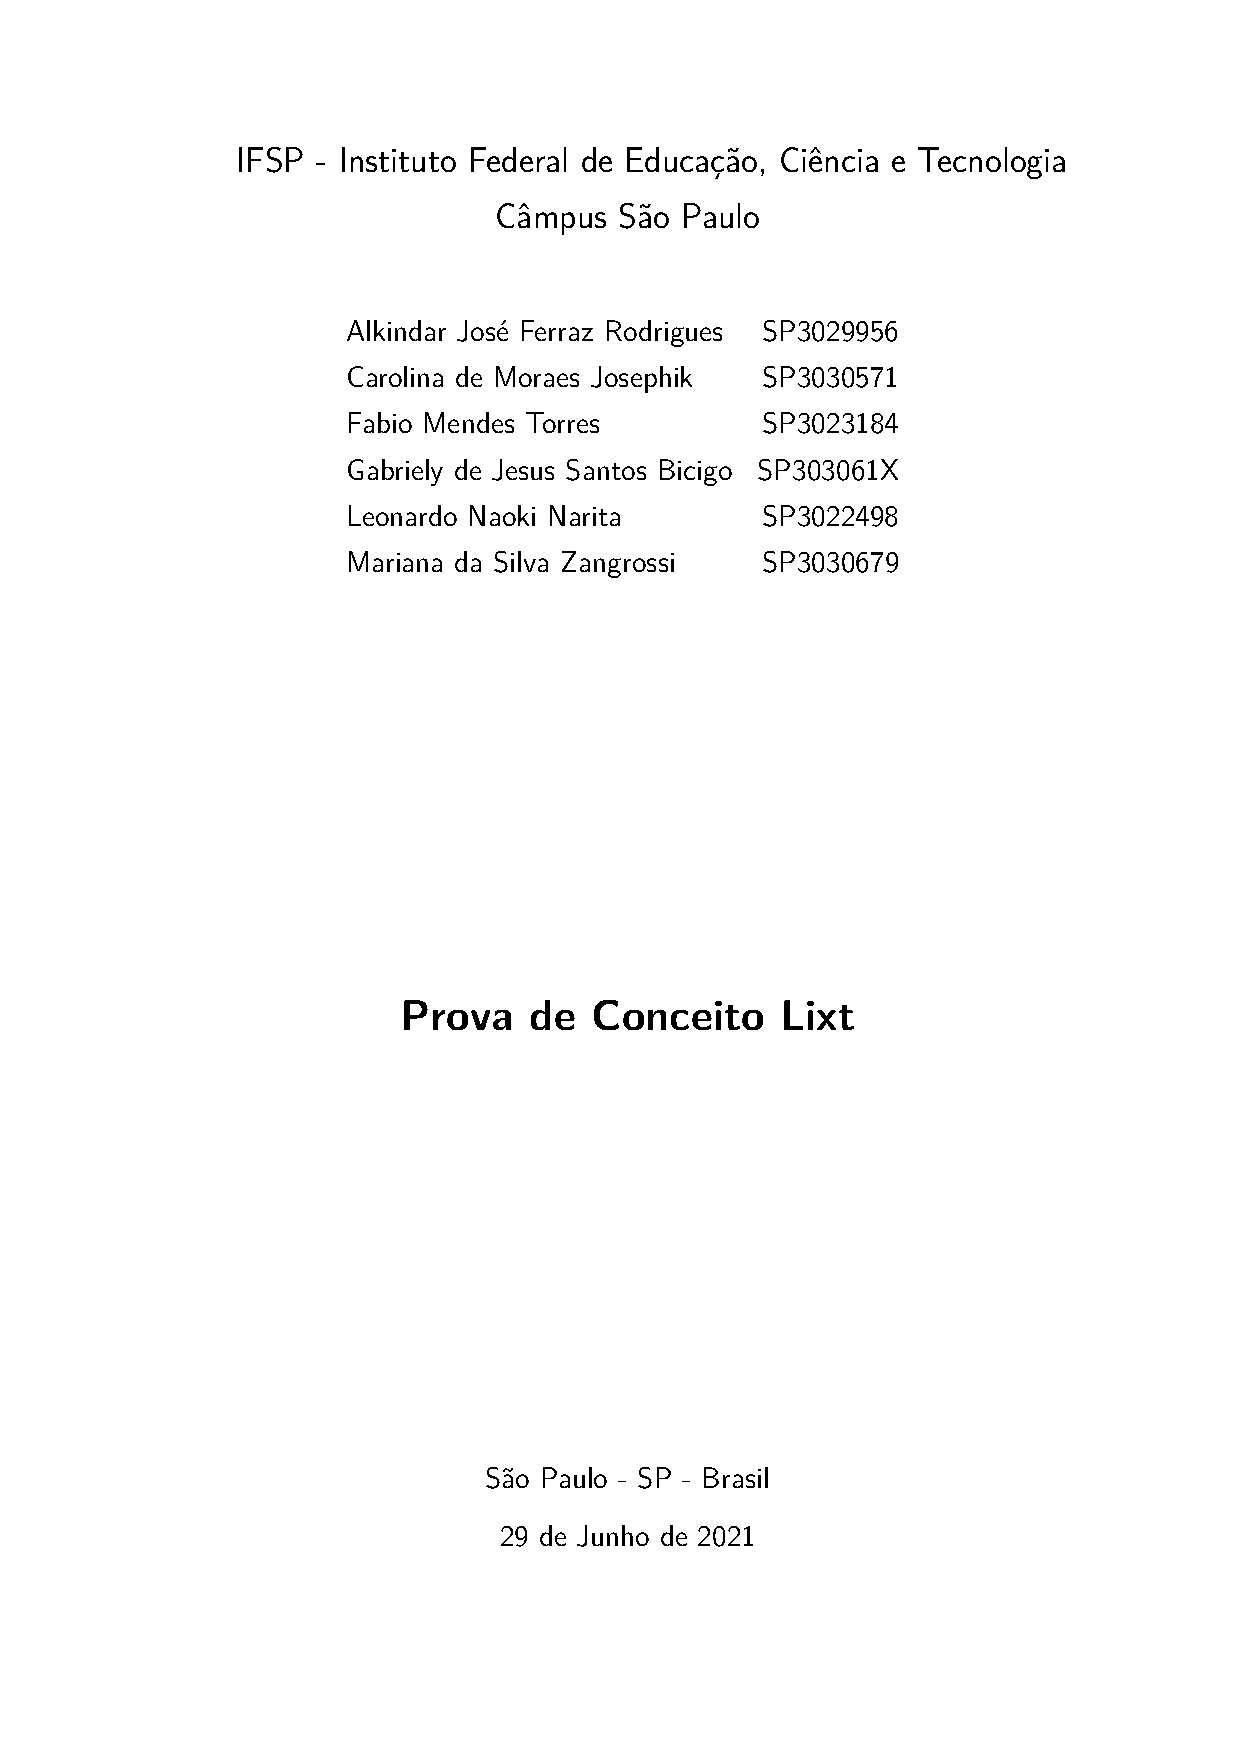
\includepdf[pages=1,scale=0.7,frame=true,pagecommand=\chapter{Prova de Conceito}\label{poc}]{apendices/poc.pdf}
\includepdf[pages=2-9,scale=0.8,frame=true,pagecommand={}]{apendices/poc.pdf}
% ----------------------------------------------------------

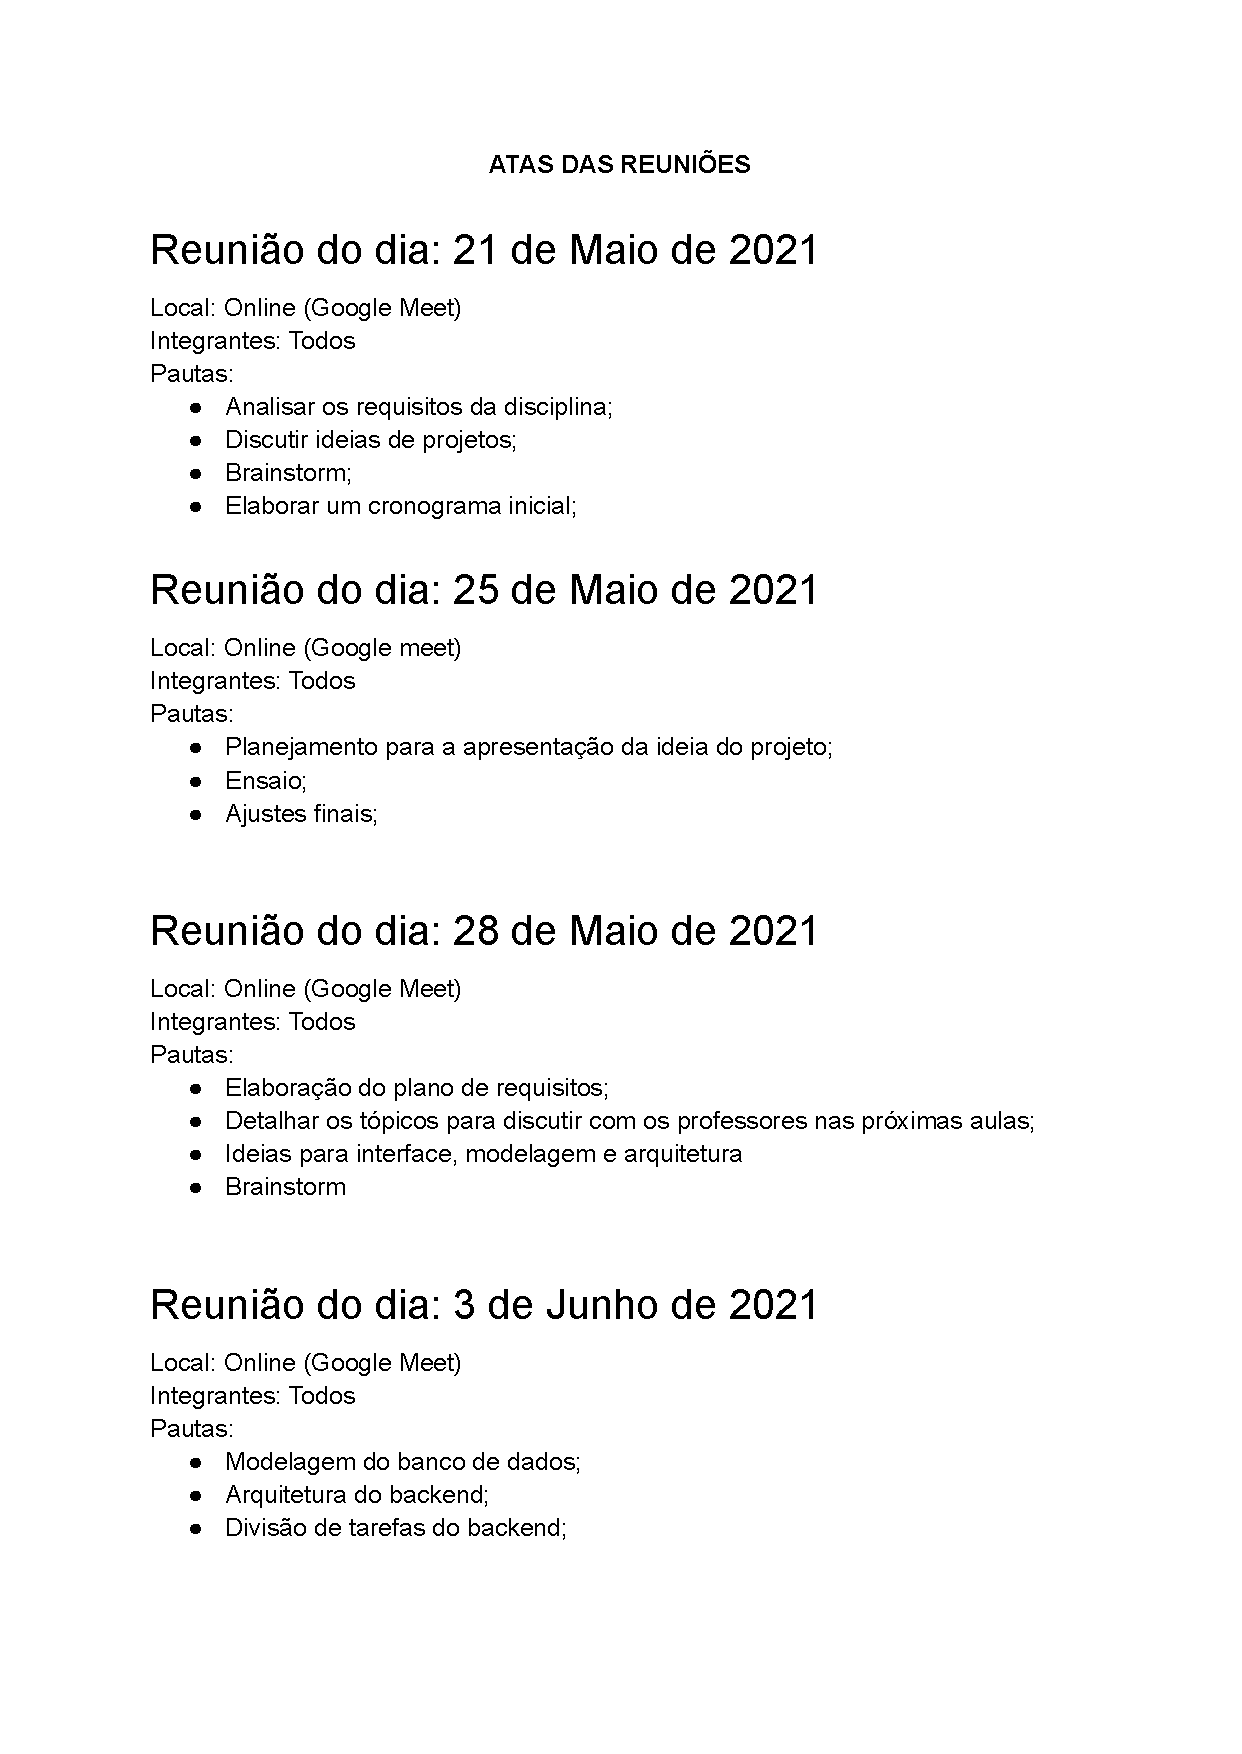
\includepdf[pages=1,scale=0.7,frame=true,pagecommand={\chapter{Atas das Reuniões}}]{apendices/atas_das_reunioes.pdf}
\includepdf[pages=2-4,scale=0.8,frame=true,pagecommand={}]{apendices/atas_das_reunioes.pdf}

\chapter{Publicações do Blog}

Nossa equipe criou o blog chamado Equipe \gls{tgt}, onde semanalmente um dos membros da equipe criava uma postagem referente a como foi a semana anterior. Nesse apêndice estão as publicações que colocamos no blog.\\

\textbf{Título}: 1° Semana do projeto

\textbf{Data da publicação}: 24 de maio de 2021

\textbf{Autora}: Gabriely

A primeira semana da equipe \gls{tgt} foi marcada por diversas reuniões de alinhamento. Essas conversas foram de extrema importância para a sondagem de conhecimentos técnicos que cada um do grupo possui e para o brainstorm da aplicação a ser desenvolvida. Foram realizados dois \textit{checkpoints} essenciais: o de distribuição de tarefas referentes a proposta que deve ser entregue no dia 25/05/2021 e o de validação de andamento da proposta, para garantir que tudo está devidamente feito, formatado, e adequado para a apresentação. A cada dia o projeto se torna mais real, o que gera uma ansiedade boa... e ruim também. Que comecem os jogos! \\

\protect\rule{13cm}{.5pt}
\\

\textbf{Título}: 2ª Semana do projeto

\textbf{Data da publicação}: 30 de maio de 2021

\textbf{Autora}: Mariana

Após nossa apresentação da proposta inicial no dia 25/05, ficamos mais aliviados com os \textit{feedbacks} dos professores. Um desses \textit{feedbacks} foram referentes à modelagem dos dados pertinentes da nossa aplicação, mas no fim, nossa proposta foi aceita.

Na sexta-feira, dia 29/05, nos reunimos novamente através da plataforma Google Meet para compartilharmos progressos que alguns integrantes já tinham feito, como esboços do aplicativo, ideias para apresentação de dados através de gráficos, e uma modelagem inicial dos dados. Além disso, tivemos alguns momentos de \textit{brainstorm} para trazer novas ideias e começamos a decidir quais \textit{features} poderiam ser deixadas para a versão 2.0, que seriam para o próximo semestre. Por fim, nesta reunião, decidimos que iríamos começar a fechar o escopo, ou seja, definir de fato o que vamos trabalhar nesse semestre, e começar a ter menos \textit{brainstorm} na equipe. Para que possamos concordar com o fechamento de escopo, criamos um documento no Google Docs, para listar todas as funcionalidades com o maior detalhamento possível, e para tirarmos dúvidas sobre esses detalhes. Assim, podemos começar a focar no que será entregue neste semestre! $\backslash$o/

É isso, até a próxima! \\

\protect\rule{13cm}{.5pt}
\\

\textbf{Título}: 3ª Semana do Projeto

\textbf{Data da publicação}: 8 de junho de 2021

\textbf{Autor}: Fabio

Depois de termos feito o levantamento de ideias, feito os esboços de modelagem e começado a delimitar o escopo mostramos para os professores no início dessa 3ª semana.

Os professores deram um \textit{feedback} positivo e mostraram os pontos que precisávamos rever na modelagem e escopo. Depois dessa reunião focamos em fazer as modificações necessárias para a versão final do escopo e modelagem, além de formalizar isso no documento do desenho de aplicação.

Resumindo foi uma semana bem cheia fizemos umas duas reuniões de alinhamento em equipe pelo Google Meet (uma delas com mais de duas horas de duração) e várias horas fazendo diagramas, resolvendo problemas, e pesquisando pra resolver dúvidas que apareciam. Mas no final das contas conseguimos avanços significativos.

Que venha a próxima semana!\\

\protect\rule{13cm}{.5pt}
\\

\textbf{Título}: 4ª Semana do Projeto

\textbf{Data da publicação}: 16 de junho de 2021

\textbf{Autor}: Alkindar

Nesta quarta semana de projeto ainda estávamos construindo o desenho da aplicação que foi entregue no dia 08/06. Para a construção do documento dividimos nas seguintes seções:\\



Introdução: Mariana

Planejamento do projeto: Gabi

Revisão bibliográfica: Mariana

Arquitetura: Alkindar

Escopo: Fábio 

Viabilidade financeira: Leonardo 

Escalabilidade: Alkindar

Critérios de segurança, privacidade e legislação: Fábio

Tecnologias a serem utilizadas: Carolina

Manutenibilidade da aplicação desenvolvida: Alkindar \\



Dificuldades com o \LaTeX \space a parte, diversos desdobramentos e detalhes da implementação da aplicação dos quais ainda não possuíamos de forma clara foram definidos. Infelizmente descobrimos que o modelo que utilizamos para criar o documento não era o correto, isso acarretará na correção do documento para o \textit{layout} correto. No final dessa semana também iniciamos a criação da apresentação do desenho da aplicação que foi realizada no dia 15/06.

Outros avanços obtidos essa semana:

Conseguimos configurar o Gource para gerar os vídeos do projeto. 

Organizamos os repositórios de desenvolvimento da aplicação no Github. 

A parte de autenticação do usuário no \textit{\gls{backend}} já está em desenovlvimento.

O \textit{boilerplate} da aplicação \textit{mobile} já está no repositório do \textit{mobile}\\



Estamos suando a camisa, galera. Mas bora para a próxima semana! \\

\protect\rule{13cm}{.5pt}
\\

\textbf{Título}: 5ª Semana do Projeto

\textbf{Data da publicação}: 25 de junho de 2021

\textbf{Autor}: Alkindar

Dado o \textit{feedback} menos que ideal dos professores diante do nosso desenho de projeto, optamos por incluir uma tarefa a mais na \textit{\gls{sprint}} inicial: reescrever o documento de forma a satisfazer as demandas dos professores.

Com esta nova tarefa, a equipe adotou uma estratégia de dividir e conquistar. Depois de avaliar os pontos que precisam ser melhorados do documento, uma parte da equipe focou em reescrevê-lo, enquanto outra parte encaminou o desenvolvimento necessário para a apresentação da prova de conceito, com as tarefas desta primeira \textit{\gls{sprint}}.

Focaram no documento:

\begin{itemize}
			\item Alkindar, Gabriely e Mariana.
\end{itemize}

Desenvolver as primeiras funcionalidades da aplicação:

\begin{itemize}
			\item Carolina, Fábio e Leonardo.
\end{itemize}

Seguimos cumprindo o calendário de \textit{\gls{sprint}}, realizando as cerimônias. Quando o documento for finalizado a equipe inteira focará nas funcionalidades desta \textit{\gls{sprint}}.\\

\protect\rule{13cm}{.5pt}
\\

\textbf{Título}: 6º semana do projeto

\textbf{Data da publicação}: 29 de junho de 2021

\textbf{Autora}: Gabriely

 A 6º semana foi marcada por um ritmo de desenvolvimento intenso para que, na apresentação na da \gls{poc} tudo estivesse de acordo com a expectativa alinhada pelo time. 

Para tal, a infraestrutura deveria ser construída e os times de \textit{\gls{backend}} e \textit{\gls{frontend}} deveriam trabalhar em conjunto para entregar as funcionalidades definidas para essa etapa.

Os desafios e dificuldades foram muitos, porém a cada conquista o time celebrava e comemorava. Essa semana reforçou nosso engajamento e nos mostrou desafios reais de um desenvolvimento real. Avante! \\

\protect\rule{13cm}{.5pt}
\\

\textbf{Título}: 7º Semana do Projeto

\textbf{Data da publicação}: 5 de julho de 2021

\textbf{Autor}: Leonardo

Essa semana apresentamos a \gls{poc} do projeto, apresentando o \textit{\gls{backend}}, \textit{\gls{frontend}}, infraestrutura, tecnologias e arquiteturas utilizadas. Ainda que tenham ocorrido contratempos durante a apresentação, o resultado avaliado pelos professores foi satisfatório, apontando apenas alguns pontos de melhoria na infraestrutura.

No decorrer da semana, houveram várias atividades em paralelo sendo executadas, tais como início do planejamento da documentação do projeto para a entrega no dia 13/07, o desenvolvimento inicial dos \textit{endpoints} das segunda \textit{\gls{sprint}}, o planejamento de validações de segurança na \gls{api}, a criação das primeiras telas no \textit{\gls{frontend}}, planejamento e organização de testes automatizados (tanto no \textit{\gls{backend}} quanto no \textit{\gls{frontend}}) e configuração de \gls{https} na \gls{aws}.

Faltando praticamente um mês para a finalização do semestre, estamos todos frenéticos para as entregas finais. Vamos com tudo!\\

\protect\rule{13cm}{.5pt}
\\

\textbf{Título}: 8º Semana do Projeto

\textbf{Data da publicação}: 13 de julho de 2021

\textbf{Autor}: Fabio

Essa semana foi muito corrida, com as data da entrega final se aproximando todos tiveram que acelerar o ritmo para manter tudo dentro do prazo planejado.

Seguimos com o desenvolvimento das funcionalidades que vamos implementar para a entrega do \gls{mvp} que incluem o compartilhamento das listas e o gerenciamento dos convites, na implementação dessas funcionalidades e no plano de testes. Também trabalhamos procurando soluções para alguns problemas no \textit{\gls{backend}} com a hospedagem da aplicação, mas temos tido êxito em contornar esses imprevistos.

Outra parte importante dessa semana foi continuar a compilação de tudo que foi produzido de documentação desde a primeira semana de projeto até agora no documento final que vamos entregar com o \gls{mvp}.

Não tem sido fácil conciliar trabalho, as tarefas da disciplina de Projeto Integrado e de todas as demais disciplinas, mas seguimos firmes, rumo a reta final! \\

\protect\rule{13cm}{.5pt}
\\

\textbf{Título}: 9º Semana do Projeto

\textbf{Data da publicação}: 23 de julho de 2021

\textbf{Autor}: Gabriely

A cada dia mais próximos da entrega final o grupo se encontra engajado em solucionar os pontos de desenvolvimento pendentes. Após a entrega da documentação do \gls{mvp} pudemos dedicar total energia a codificação e pesquisa de soluções que atendessem nossas necessidades e resolvessem nossos dilemas. O ritmo tem sido intenso para combinar com nossa ansiedade e a cada semana superada nos surpreendemos com como conseguimos conciliar todos os ``pratinhos'' ao mesmo tempo. Talvez, em quesito técnico, não sejamos nenhum Mark Zuckerberg, mas só por conseguirmos lidar com a vida pessoal, profissional e acadêmica no meio de uma PANDEMIA enquanto saímos das nossas zonas de conforto técnicas para entregar o melhor, somos incríveis! Fica aqui meus parabéns a cada um da equipe. Avante! \\

\protect\rule{13cm}{.5pt}
\\

\textbf{Título}: 10º Semana do Projeto

\textbf{Data da publicação}: 3 de agosto de 2021

\textbf{Autor}: Mariana

Com a chegada de final de semestre e da apresentação do nosso MVP, na última semana, estivemos focando em vários aspectos para entregar um \gls{mvp} consistente com o que propomos anteriormente. Primeiramente, nos encontramos diversas vezes durante a semana, para treinar e ensaiar a nossa apresentação através de um documento powerpoint, separando cada fala para cada integrante, além de contabilizar o tempo e tentar achar gaps que pudesse ser melhorados na apresentação final. Além disso, essa semana tivemos muita troca de suporte e ajuda, para superar desafios que surgiram de último momento. Enquanto tudo isso acontece, o documento final do mvp está sendo desenvolvido, para ser entregue na semana que vem. \\

\protect\rule{13cm}{.5pt}
\\

\textbf{Título}: 11ª Semana do Projeto -- Retomada de férias

\textbf{Data da publicação}: 29 de setembro de 2021

\textbf{Autor}: Alkindar

Nesta semana, de retomada de férias, a equipe voltou a atuar com foco e força no projeto, acelerando o ritmo em relação ao que foi desenvolvido nas férias. Durante o recesso de meio de ano, corrigimos alguns apontamentos indicados pelos professores, como 

\begin{itemize}
	\item salvar tokens de acesso no banco,
	\item alterar a terminologia: "deletar lista" para "excluir lista",
	\item confirmar a exclusão de listas, 
	\item entre outros.
\end{itemize}

Com estas tarefas em vias de finalização, e apresentadas aos professores no dia 23 de setembro, iniciamos o planejamento das funcionalidades que serão implementadas nesta segunda fase do projeto, a divisão das \textit{\glspl{sprint}} e quebra das tarefas que comporão cada uma.  Uma cronograma estimado será apresentado no próximo encontro com os professores, no dia 30 de setembro. \\

\protect\rule{13cm}{.5pt}
\\

\textbf{Título}: 12ª Semana do projeto

\textbf{Data da publicação}: 4 de outubro de 2021

\textbf{Autor}: Carolina

Durante esta semana finalizamos o planejamento e a criação do cronograma o apresentamos dia 30/09 para os professores. Conforme o \textit{feedback} da apresentação realizada nós temos itens a corrigir.

O nosso cronograma pode ser visualizado no link abaixo:

[A6PGP] Index of /S202101-PI/TGT/Documentos/Planejamento (ifsp.edu.br)

As correções solicitadas foram:

\begin{itemize}
	\item Não demarcar uma data limite para cada tarefa uma vez que isso iria de contramão ao SCRUM (metodologia que estamos utilizando);
	\item Não alocar qual recurso fará cada tarefa uma vez que no SCRUM entende-se que quem estiver disponível pode pegar a tarefa que estiver no backlog;
	\item Estabelecer o cronograma visando a finalização no dia 18/11.
\end{itemize}

Além do planejamento, prosseguimos com o desenvolvimento do \textit{\gls{backend}} e do \textit{\gls{frontend}} adiantando o início das tarefas que compõe a primeira \textit{\gls{sprint}} documentada no cronograma. \\

\protect\rule{13cm}{.5pt}
\\

\textbf{Título}: 13° Semana do projeto

\textbf{Data da publicação}: 7 de outubro de 2021

\textbf{Autor}: Fabio

Ao longo dessa semana fizemos as correções que os professores sugeriram quando apresentamos nosso planejamento até a entrega final. Além disso, continuamos com o desenvolvimento das tarefas da \textit{\gls{sprint}} atual e conseguimos concluir: 

\begin{itemize} 
	\item A melhoria do fluxo de redefinição de senha: o usuário não recebe mais uma senha aleatória e válida gerada pelo sistema, mas um link para um formulário onde ele deve inserir uma nova senha (tudo validado por tokens JWT); 
	\item A implementação dos comentários globais no front-end: Com essa funcionalidade os usuários podem acrescentar um comentário em um item que aparece em todas as listas de compras, para não ter que inserir um mesmo comentário sempre que acrescenta um item a uma nova lista;
\end{itemize}

Também tivemos nossa reunião semanal com os professores e pudemos retirar dúvidas sobre os certificados de segurança exigidos para a aplicação, mostrar as novas funcionalidades implementadas para validação e relatar as correções no planejamento. O \textit{feedback} dos professores foi positivo e as sugestões de melhorias foram muito relevantes.
Ao longo dessa semana também dedicamos um tempo para verificar o que deve ser atualizado na documentação para evitar acumular trabalho para o final do semestre.

Nessa semana foi isso. Até a próxima semana!! \\

\protect\rule{13cm}{.5pt}
\\

\textbf{Título}: 14º Semana do projeto

\textbf{Data da publicação}: 14 de outubro de 2021

\textbf{Autor}: Gabriely

 Tivemos mais uma semana superada dentro do projeto. Nela, a equipe iniciou algumas das atividades presentes em nosso backlog do Trello e também concluiu atividades que já estavam em andamento. 

\begin{itemize}
	\item Os testes de tela do \textit{\gls{frontend}}, que estavam em aberto, foram concluídos com sucesso;
	\item Foi iniciado o desenvolvimento da funcionalidade de geolocalização, para detectar o estabelecimento onde o cliente está realizando a compra; 
	\item A parte de infraestrutura passou por alterações que auxiliaram na melhoria das métricas de segurança, O próximo passo, agora, é medir o quanto isso limita a nossa base de usuários para que seja possível decidir em que ponto deixaremos a segurança; 
	\item A feature de comentário global segue sendo desenvolvida pelo time.
\end{itemize}

Também foi realizada a reunião semanal com os professores, onde pudemos compartilhar o andamento do projeto e tirar algumas dúvidas sobre as atividades. 

Estamos prontos para a próxima semana! Até a próxima \\

\protect\rule{13cm}{.5pt}
\\

\textbf{Título}: 15º Semana do Projeto

\textbf{Data da publicação}: 22 de outubro de 2021

\textbf{Autor}: Leonardo

Nessa semana, prosseguimos no desenvolvimento do projeto atuando na \textit{\gls{sprint}} 07.

\begin{itemize}
	\item Foi finalizado o fluxo base da Geolocalização no \textit{\gls{backend}} tratando erros e com testes automatizados planejados;
	\item Foi iniciada a feature de código de barras no \textit{\gls{frontend}};
	\item Tiramos as métricas do projeto (Linhas de código, commits, classes, etc);
	\item Foi continuado o processo de melhoria de metricas de segurança na infraestrutura;
	\item Houve, no dia 20/10/2021, um refining (cerimônia \textit{\gls{scrum}} para entender a regra de negócio de uma demanda) sobre os módulos de Histórico e Análise de Compras no Lixt.
\end{itemize}

Essa semana, devido ao Conselho Pedagógico para os Cursos Técnicos, não tivemos uma conexão direta com os professores orientadores do projeto. Contudo, estamos com toda energia para finalizar o projeto.

Vamos com tudo! \\

\protect\rule{13cm}{.5pt}
\\

\textbf{Título}: 16º Semana do Projeto

\textbf{Data da publicação}: 7 de novembro de 2021

\textbf{Autor}: Mariana

Na semana 16 (18/10 a 22/10), não tivemos aulas, o que nos deu a oportunidade de focar mais no desenvolvimento do Lixt. Durante a semana pudemos:

\begin{itemize}
	\item Nos reunir para discutir como poderíamos mostrar as análises de forma amigável e prática ao usuário, além da localização e histórico de compras;
	\item Discutimos sobre a funcionalidade de comentários globais, se eles deveriam ser públicos ou privados e nos marcamos de nos encontrar para discutir isso de forma mais aprofundada e técnica;
	\item No \textit{\gls{frontend}}, estávamos desenvolvendo o cadastro de produto com código de barras, além da criação de testes unitários para o leitor de código de barras.
\end{itemize}

Estamos cada dia chegando mais perto da entrega, e durante esse período, estamos tirando todas as dúvidas possíveis com os professores, além de mostrá-los como está o andamento das funcionalidades finais.

É isso! Até a próxima semana.  \\

\protect\rule{13cm}{.5pt}
\\

\textbf{Título}: 17º Semana do Projeto

\textbf{Data da publicação}: 8 de novembro de 2021

\textbf{Autor}: Alkindar

Nesta semana (23 a 30/10), demos continuidade ao desenvolvimento do projeto. Como colocado no último post, aproveitamos que na semana anterior não tivemos aula aumentar o foco no planejamento das últimas features a serem desenvolvidas, principalmente as questões de análises estatísticas, geolocalização e código de barras. 

As queries para extrair os dados, após serem definidas, começaram a ser implementadas no \textit{\gls{backend}}, e em breve estarão disponíveis no app com visualizações amigáveis para o usuário. Em paralelo, a questão dos comentários globais está avançando. 

Também no \textit{\gls{backend}} foi implementada uma flag no comentário para avisar se é um comentário público ou não, assim como um filtro, para evitar vulnerabilidades que exponham o conteúdo de todos os comentários para todos os usuários. Como ainda falta implementar a ordenação dos comentários no \textit{\gls{frontend}}, e isso requer mais flags a entidade usuário, os testes serão reescritos após finalizarmos esta feature, já que alterar a entidade usuário requer alterar todos os testes que temos. No \textit{\gls{frontend}}, a visualização básica dos comentários globais foi implementada, faltando apenas ordenar de acordo com a preferência do usuário.

Além disso, no \textit{\gls{frontend}}, seguindo recomendações dos professores, duas alterações foram feitas:

\begin{itemize}
	\item O app passa as coordenadas reais do usuário para que esta informação seja salva em banco, e o entendimento do local onde o usuário se encontra, em termos de nome e endereço é feito no \textit{\gls{backend}}.
	\item Foram feitas algumas alterações no processo de leitura do código de barras, a começar pelo ícone que indica esta funcionalidade:
		\begin{itemize}
		\item Ao cadastrar um produto já existente, o app sugere o produto para o usuário;
		\item O código de barras pode ser digitado, para casos em que a leitura via câmera não funciona (este modo de busca exigiu uma pequena mudança no \textit{\gls{backend}} também).
		\end{itemize}
\end{itemize} 

Este foi o andamento nesta última semana, estamos tão perto mas tão longe de finalizarmos... Uma hora chegamos lá \\

\protect\rule{13cm}{.5pt}
\\

\textbf{Título}: 18ª semana de projeto

\textbf{Data da publicação}: 14 de novembro de 2021

\textbf{Autor}: Carolina

Na 18ª semana de projeto, demos prosseguimento ao desenvolvimento das tarefas do cronograma além dos ajustes solicitados pelos professores nas conversas semanais.

Esta semana foi completada a funcionalidade de alteração do status (privado ou público) do comentário global, correções na interface de comentários e testes da mesma. Além disso, a tela de histórico de compras também foi desenvolvida e testada.

No \textit{\gls{backend}} ajustes dos comentários globais também foram realizados: filtragem dos comentários globais no servidor para evitar vulnerabilidade e implementação da flag de para preferência de ordenação. Além disso, foi dado prosseguimento nas tarefas relativas às queries da funcionalidade de estatísticas.

Quanto à documentação, foram realizadas revisões e correções do documento para a adequação ao modelo proposto na disciplina.

Este foi o progresso da 18ª semana de projeto. Estamos chegando ao fim e se tudo der certo significa que estamos próximos dos últimos relatórios de progresso também

Até mais!

%\chapter{Manual Técnico}

%\section{Arquitetura}
%\todonum[inline]{Copiar a arquitetura do desenho da aplicações (com os ajustes que forem necessários}

%\section{Modelagens e Definições Técnicas}
%\todonum[inline]{Copiar a seção Modelagens e definições do desenho da aplicação (com os ajustes que forem necessários}

%\section{Tecnologias Utilizadas}
%\todonum[inline]{Copiar as Tecnologias Utilizadas do desenho da aplicação}

%\section{Diagramas de Sequência}
%\todonum[inline]{Criar os diagramas de sequencia}

%\section{Diagramas de Classes}
%\todonum[inline]{Criar os diagramas de classes}

%\chapter{Manual do Usuário}
%\todonum[inline]{Criar o manual do usuário}

%\chapter{Política de Privacidade}
%Essa página pretende informar os Usuários de nossa aplicação sobre nossas políticas e procedimentos sobre coleta, uso e divulgação das informações coletadas durante o uso de nossos serviços e informa sobre seus direitos de privacidade e como a lei o protege.

Ao optar por utilizar nossos serviços, você concorda com a coleta e uso de informações em relação a esta política. As informações pessoais coletadas são utilizadas para fornecer e melhorar o serviço. Essas informações não serão compartilhadas com ninguém, exceto conforme descrito nesta Política de Privacidade.

Os termos usados nesta Política de Privacidade têm os mesmos significados que nossos Termos e Condições, que podem ser acessados no aplicativo Lixt, a menos que definido de outra forma nesta Política de Privacidade.

\section{Termos, Definições e Interpretação}
\subsection{Interpretação}

As palavras cuja letra inicial é maiúscula têm significados definidos nas seguintes condições. As seguintes definições devem ter o mesmo significado, independentemente de aparecerem no singular ou no plural.

\subsection{Termos e Definições}

Para os propósitos dessa política de privacidade:

\begin{itemize}
	\item \textbf{Conta} significa a conta única criada pelo Usuário para acessar nossos serviços ou partes deles.
	\item \textbf{Aplicação} se refere ao software denominado Lixt, desenvolvido e disponibilizado pela Equipe TGT, pelo Usuário em qualquer dispositivo eletrônico.
	\item \textbf{Empresa} (referenciada como "Nós", "Equipe", ou "Equipe TGT" neste documento) refere-se ao aplicativo Lixt.
	\item \textbf{País} refere-se ao Brasil
	\item \textbf{Dispositivo} significa qualquer dispositivo que pode acessar o serviço como computadores, celulares ou tablet's.
	\item \textbf{Dados Pessoais} são quaisquer informações relacionadas a um indivíduo identificado ou identificável.
	\item \textbf{Serviço} se refere à aplicação.
	\item \textbf{Provedor de Serviço} se refere a qualquer pessoa física ou jurídica que processa dados em nome da Empresa. Refere-se a empresas terceirizadas ou indivíduos contratados pela Empresa para facilitar o mantenimento da Aplicação, para fornecer o Serviço em nome da Empresa, para realizar serviços relacionados ao Aplicativo Lixt ou para auxiliar-nos na análise de como os Serviços prestados pela Empresa são utilizados.
	\item \textbf{Dados de Uso} Os Dados de Uso referem-se aos dados coletados automaticamente, sejam gerados pelo uso do Serviço ou da própria infraestrutura do Serviço.
	\item \textbf{Usuário} Significa o indivíduo que acessa ou usa o Serviço, ou a empresa ou outra pessoa jurídica em nome da qual tal indivíduo está acessando ou usando o Serviço, conforme aplicável.
	\item \textbf{Terceiros} Empresas ou indivíduos sem relação direta com a Equipe TGT.
\end{itemize}

\section{Coleta e Uso de Dados Pessoais}
\subsection{Tipos de Dados Coletados}

Ao usar nosso serviço, podemos solicitar que você nos forneça certas informações de identificação pessoal que podem ser usadas para contatá-lo ou identificá-lo. As informações de identificação pessoal podem incluir, mas não se limitam a:

\begin{itemize}
	\item Nome
	\item Informações de contato (endereço eletrônico)
	\item Localização: para fornecer algumas funcionalidades de nosso aplicativo, sua localização pode ser coletada com sua permissão prévia. Essa informação pode ser armazenada nos servidores da Empresa, servidor de um Provedor de Serviços ou podem ser simplesmente armazenadas em Seu dispositivo. Você pode ativar ou desativar o acesso a essas informações a qualquer momento, por meio das configurações do seu dispositivo.
	\item Lista de contatos
	\item Conteúdos compartilhados com amigos (no escopo da aplicação)
	\item Bens adquiridos, data, local e valor de compra
\end{itemize}

\subsection{Dados de Uso Coletados}

\begin{itemize}
	\item Dados de Log: Ao utilizar o Serviço, em caso de erro no aplicativo, são coletados dados e informações (através de produtos de Terceiros) no seu telefone chamados Logs. Esses dados de registro podem incluir informações como endereço de protocolo de Internet ("IP") do dispositivo, nome do dispositivo, versão do sistema operacional, configuração do aplicativo ao utilizar meu serviço, hora e data de uso do serviço e outras estatísticas.
\end{itemize}

\subsection{Uso dos Dados Pessoais Coletados}

A Empresa pode coletar dados com os seguintes propósitos:

\begin{itemize}
	\item \textbf{Prover ou manter Nossos Serviços} incluindo monitorar o uso dos Serviços prestados.
	\item \textbf{Para gerenciar as Contas dos Usuários:} Para registrar um indivíduo como Usuário do Serviço. As Informações Pessoais coletados permitem acesso a diferentes funcionalidades no aplicativo disponíveis apenas a usuários registrados.
	\item \textbf{Para entrar em contato:} unicamente via email ou notificações pelo aplicativo Lixt. Para informá-lo sobre atualizações, informativos de nocas funcionalidades, produtos ou serviços, incluindo atualizações de segurança e/ou privacidade, quando necessário.
	\item \textbf{Para prover aos Usuários:} Ofertas especiais e informações gerais sobre outros bens, serviços e eventos que oferecemos semelhantes aos que você já comprou ou perguntou, a menos que você tenha optado por não receber tais informações.
	\item \textbf{Para gerenciar suas solicitações:} atender e gerenciar seus pedidos para nós.
	\item \textbf{Para transferências de negócios:} as informações dos Usuários podem ser usadas para avaliar ou conduzir uma fusão, alienação, reestruturação, reorganização, dissolução ou outra venda ou transferência de alguns ou todos os nossos ativos, seja em continuidade ou como parte de falência, liquidação, ou procedimento similar, no qual os Dados Pessoais que possuímos sobre os usuários do nosso Serviço estejam entre os ativos transferidos.
	\item \textbf{Para outros propósitos:} as informações coletados podem ser usadas para outros fins, como análise de dados, identificação de tendências de uso, determinação da eficácia de nossas campanhas promocionais e para avaliar e melhorar nosso serviço, produtos, serviços, marketing e sua experiência. 
\end{itemize}

Suas informações podem ser compartilhadas nas seguintes situações:

\begin{itemize}
	\item \textbf{Com Provedores de Serviços:} Podemos compartilhar suas informações pessoais com provedores de serviços para monitorar e analisar o uso de nosso serviço, e/ou entrar em contato com Usuários.
	\item \textbf{Para transferências de negócios:} As informações dos Usuários podem ser usadas para avaliar ou conduzir uma fusão, alienação, reestruturação, reorganização, dissolução ou outra venda ou transferência de alguns ou todos os nossos ativos, seja em continuidade ou como parte de falência, liquidação, ou procedimento similar, em que os Dados Pessoais que possuímos sobre os usuários do nosso Serviço estejam entre os ativos transferidos.
	\item \textbf{Com afiliados:} nesse caso, exigiremos que essas afiliadas honrem esta Política de Privacidade. Afiliadas incluem Nossa empresa-mãe e quaisquer outras subsidiárias, parceiros de união de risco ou outras empresas que controlamos ou que estão sob controle comum conosco.
	\item \textbf{Com parceiros de negócios:} podemos compartilhar suas informações com nossos parceiros de negócios para oferecer a você determinados produtos, serviços ou promoções.
	\item \textbf{Com outros usuários:} quando você compartilha informações pessoais ou de outra forma interage nas áreas públicas com outros usuários, tais informações podem ser visualizadas por todos os usuários e podem ser distribuídas publicamente fora do aplicativo.
	\item \textbf{Com seu consentimento:} podemos divulgar suas informações pessoais para qualquer outra finalidade.
\end{itemize}

\subsection{Período de Armazenamento dos Dados Coletados}

A Empresa reterá Seus Dados Pessoais apenas pelo tempo necessário para os fins definidos nesta Política de Privacidade. Reteremos e usaremos Seus Dados Pessoais na medida necessária para cumprir nossas obrigações legais (por exemplo, se formos obrigados a reter seus dados para cumprir as leis aplicáveis), resolveremos disputas e faremos cumprir nossos acordos e políticas legais.

A Empresa também reterá os Dados de Uso para fins de análise interna. Os Dados de Uso são geralmente retidos por um período mais curto, exceto quando esses dados são usados para fortalecer a segurança ou para melhorar a funcionalidade do Nosso Serviço, ou se formos legalmente obrigados a reter esses dados por períodos mais longos.

\subsection{Transferência dos Dados Coletados}

Suas informações, incluindo Dados Pessoais, são processadas nos escritórios operacionais da Empresa e em quaisquer outros locais onde as partes envolvidas no processamento estejam localizadas. Isso significa que essas informações podem ser transferidas para - e mantidas em - computadores localizados fora do Seu estado, província, país ou outra jurisdição governamental onde as leis de proteção de dados podem ser diferir daquelas da Sua jurisdição.

O seu consentimento com esta Política de Privacidade, seguido do envio de tais informações, representa a sua concordância com essa transferência.

A Empresa tomará todas as medidas razoavelmente necessárias para garantir que Seus dados sejam tratados com segurança e de acordo com esta Política de Privacidade e nenhuma transferência de Seus Dados Pessoais ocorrerá para uma organização ou um país, a menos que haja controles adequados em vigor, incluindo a segurança de Seus dados e outras informações pessoais.

\subsection{Divulgação de Dados Coletados}

\subsubsection{Transações de Negócios}

Se a Empresa estiver envolvida em uma fusão, aquisição ou venda de ativos, Seus Dados Pessoais podem ser transferidos. Avisaremos antes que Seus Dados Pessoais sejam transferidos e se tornem sujeitos a uma Política de Privacidade diferente.

\subsubsection{Questões Legais}

Sob certas circunstâncias, a Empresa pode ser obrigada a divulgar Seus Dados Pessoais se for obrigada a fazê-lo por lei ou em resposta a solicitações válidas por autoridades públicas (por exemplo, um tribunal ou agência governamental).

\subsubsection{Outros Requisitos Legais}

A Empresa pode divulgar Seus Dados Pessoais acreditando de boa-fé que tal ação é necessária para:

\begin{itemize}
	\item Cumprir obrigações legais
	\item Proteger e defender os direitos ou Propriedades da Empresa
	\item Prevenir ou investigar possíveis atos ilícitos particados durante o uso do Serviço
	\item Proteger a segurança pessoal dos Usuários do Serviço ou do Público
	\item Proteger-se contra responsabilização legal
\end{itemize}

\subsection{Segurança dos Dados Coletados}

A segurança dos seus dados pessoais é importante para nós, mas lembre-se de que nenhum método de transmissão pela Internet ou método de armazenamento eletrônico é 100% seguro. Embora nos esforcemos para usar meios comercialmente aceitáveis para proteger Seus Dados Pessoais, não podemos garantir sua segurança absoluta.

\section{Usuários menores de 18 anos}

Nosso serviço não se dirige a menores de 18 anos. Não coletamos intencionalmente informações de identificação pessoal de menores de 18 anos. Se você for um pai ou responsável e estiver ciente que seu filho nos forneceu dados pessoais, por favor Contate-Nos. Se tomarmos conhecimento de que coletamos Dados Pessoais de qualquer pessoa com menos de 18 anos sem verificação do consentimento dos pais, tomaremos medidas para remover essas informações de Nossos servidores.

Se precisarmos confiar no consentimento como base legal para processar Suas informações e Seu país exigir o consentimento de um dos pais, podemos exigir o consentimento dos Seus pais antes de coletar e usar essas informações.

\section{Provedores de Serviços}

Nosso serviço pode conter links para outros sites que não são operados por nós. Se você clicar em um link de terceiros, será direcionado para o site desse terceiro. Aconselhamos fortemente que reveja a Política de Privacidade de cada site que visitar.

Não temos controle e não assumimos responsabilidade pelo conteúdo, políticas de privacidade e práticas de quaisquer sites ou serviços de terceiros.

Empresas terceirizadas e/ou indivíduos podem ser contratados pela TGT pelos seguintes motivos:

\begin{itemize}
	\item Facilitar o fornecimento ou mantenimento do Serviço
	\item Fornecer o Serviço em Nosso nome
	\item Executar processos e/ou procedimentos relacionados à atividade final
	\item Realizar a análise de uso dos Nossos Serviços
\end{itemize}

Estes terceiros informados podem ter acesso às suas Informações Pessoais. O motivo é realizar as tarefas atribuídas a eles em nosso nome. No entanto, eles são obrigados a não divulgar ou usar as informações para qualquer outra finalidade.

\section{Mudanças na Política de Privacidade}

Podemos atualizar nossa Política de Privacidade de tempos em tempos. Iremos notificá-lo de quaisquer alterações, publicando a nova Política de Privacidade nesta página.

Iremos informá-lo por mensagem eletrônica e/ou um aviso em destaque no Nosso Serviço, antes da alteração entrar em vigor e atualizar a data da "Última atualização" no topo desta Política de Privacidade.

Aconselhamos você a revisar esta Política de Privacidade periodicamente para quaisquer alterações. As alterações a esta Política de Privacidade entram em vigor quando publicadas nesta página.

\section{Fale Conosco}

Caso tenha dúvidas ou sugestões sobre esta Política de Privacidade, não hesite em entrar em contato pelo(s) canal(ais) abaixo:

\begin{itemize}
	\item Endereço eletrônico: \href{mailto:thegraduationteam@gmail.com}{thegraduationteam@gmail.com}
\end{itemize}

\chapter{Planos de Testes Automatizados}
Os testes são fundamentais tanto para garantir a manutenção do software quanto possibilitar a detecção de problemas de uma funcionalidade nova impactando em outras partes no sistema antes de subir oficialmente para o ambiente de produção. 

Além disso, o desenvolvimento de teste eficiente consegue auxiliar a documentação do software, indicando parâmetros e argumentos necessários para testar alguma funcionalidade em específica do sistema.

Com esse embasamento, é de extrema importância o planejamento de testes, que é abordado nesse apêndice.

\section{Plano de Testes no Back-end}

No \gls{backend}, foi usado o jUnit para desenvolver os testes automatizados tanto em nível unitário quanto em nível de integração.

Como boa prática, o código de teste do backend está segregado do código de produção. O código de produção está na pasta lixt-backend/src/main/java/br/com/ifsp/pi/lixt, enquanto o código de testes está na pasta lixt-backend/src/test/java/br/com/ifsp/pi/lixt

Nesta seção há quadros que representam os casos de teste agrupados por módulos do sistema. 

Apenas os endpoints de cadastro de usuário e de redefinir senha não necessitam de token.

\begin{quadro}[H]
\centering
\ABNTEXfontereduzida
\caption[Testes do Módulo 1 - Testes Unitários e Serviços Compartilhados]{Testes do Módulo 1 - Testes Unitários e Serviços Compartilhados}
\label{testes-servicos-compartilhados}
\begin{tabular}{|p{5.0cm}|p{5.0cm}|p{4.5cm}|}
  	\hline
 	\thead{Funcionalidade} & \thead{Pré-Requisito} & \thead{Resultado esperado}  \\
 	\hline
 	Enviar email com sucesso. & & Retornar true. \\
 	\hline
 	Enviar email com erro. & & Retornar false. \\
 	\hline
 	Gerar token com os dados do client. & Ter um clientID e secretID. & Gerar um basic token que, a partir dele, será criado o bearer token no serviço do OAuth2. \\
 	\hline
\end{tabular}
\legend{Fonte: Os autores}
\end{quadro}

\begin{quadro}[H]
\centering
\ABNTEXfontereduzida
\caption[Testes do Módulo 2 - Autenticação, Autorização e Usuário]{Testes do Módulo 2 - Autenticação, Autorização e Usuário}
\label{testes-autenticacao}
\begin{tabular}{|p{5.0cm}|p{5.0cm}|p{4.5cm}|}
  	\hline
 	\thead{Funcionalidade} & \thead{Pré-Requisito} & \thead{Resultado esperado}  \\
 	\hline
	Cadastrar-se no sistema. &  & Retornar status 200 e os mesmos dados da requisição com o id. \\
	\hline
	Realizar login & Ter cadastro prévio no sistema & Retornar status 200 e o token \\
	\hline
	Criar usuário já existente. & Já haver o username e/ou o email no banco de dados. & Retornar status 409. \\
   \hline
    Enviar um email com um link que, ao ser acessado, permitirá o usuário a trocar sua senha. & Retornar status 200. & \\
   \hline
   Resetar senha com usuário não encontrado. & & Retornar status 404.  \\
   \hline
   Atualizar senha escolhida pelo usuário. & Ter cadastro prévio no sistema. & Retornar status 200.  \\
   \hline
   Buscar dados do usuário através do token. & Ter cadastro prévio no sistema e possuir um token. & Retornar status 200 e os dados não sensíveis do usuário. \\
   \hline
\end{tabular}
\legend{Fonte: Os autores}
\end{quadro}

Obs: O token é fundamental não somente para acessar ao servidor, mas também para que consiga se identificar nos endpoints, tendo em vista que o token possui todos os dados do usuário (tais como id, email e username).

\begin{quadro}[H]
\centering
\ABNTEXfontereduzida
\caption[Testes do Módulo 3 - Categoria]{Testes do Módulo 3 - Categoria}
\label{testes-categoria}
\begin{tabular}{|p{5.0cm}|p{5.0cm}|p{4.5cm}|}
  	\hline
 	\thead{Funcionalidade} & \thead{Pré-Requisito} & \thead{Resultado esperado}  \\
 	\hline
	Cadastrar categoria. &  & Retornar status 200 e o dado cadastrado. \\
	\hline
	Buscar todas as categorias. &  & Retornar status 200 e os dados buscados. \\
	\hline
	Buscar categoria por id. & Ter a categoria cadastrada com o devido id. & Retornar status 200 e o dado buscado. \\
   \hline
    Atualizar categoria. & Ter a categoria cadastrada com o devido id. & Retornar status 200 e os dados atualizados. \\
	\hline
	Deletar categoria. & Ter a categoria cadastrada com o devido id. & Retornar status 200. \\
   \hline
\end{tabular}
\legend{Fonte: Os autores}
\end{quadro}

\begin{quadro}[H]
\centering
\ABNTEXfontereduzida
\caption[Testes do Módulo 4 - Produto]{Testes do Módulo 4 - Produto}
\label{testes-produto}
\begin{tabular}{|p{5.0cm}|p{5.0cm}|p{4.5cm}|}
  	\hline
 	\thead{Funcionalidade} & \thead{Pré-Requisito} & \thead{Resultado esperado}  \\
 	\hline
	Cadastrar produto. &  & Retornar status 200 e o dado cadastrado. \\
	\hline
	Buscar produto por id. & Ter a produto cadastrado com o devido id. & Retornar status 200 e o dado buscado. \\
   \hline
    Atualizar produto. & Ter a produto cadastrada com o devido id. & Retornar status 200 e os dados atualizados. \\
	\hline
	Deletar produto. & Ter a produto cadastrada com o devido id. & Retornar status 200. \\
   \hline
    Buscar por semelhança de nome. & & Retornar status 200. \\
   \hline
\end{tabular}
\legend{Fonte: Os autores}
\end{quadro}

\begin{quadro}[H]
\centering
\ABNTEXfontereduzida
\caption[Testes do Módulo 5 - Lista]{Testes do Módulo 5 - Lista}
\label{testes-lista}
\begin{tabular}{|p{5.0cm}|p{5.0cm}|p{4.5cm}|}
  	\hline
 	\thead{Funcionalidade} & \thead{Pré-Requisito} & \thead{Resultado esperado}  \\
 	\hline
	Criar lista. & & Retornar status 200 e o dado cadastrado. \\
	\hline
	Buscar lista por id. & Ter cadastro prévio da lista e ter acesso à lista. & Retornar status 200 e o dado buscado. \\
   \hline
   Buscar lista por id sem acesso. & Ter cadastro prévio da lista e não ter acesso à lista. & Retornar status 403. \\
   \hline
    Atualizar lista. & Ter a lista cadastrada com o devido id e ser dono da lista. & Retornar status 200 e os dados atualizados. \\
	\hline
	 Atualizar lista sem acesso. & Ter a lista cadastrada com o devido id e não ser dono da lista. & Retornar status 403. \\
	\hline
	Deletar lista. & Ter a lista cadastrada com o devido id e ser dono da lista. & Retornar status 200. \\
   \hline
    Deletar lista sem acesso. & Ter a lista cadastrada com o devido id e não ser dono da lista. & Retornar status 403. \\
   \hline
    Buscar listas que um usuário possui acesso. & & Retornar status 200 e os dados buscados. \\
   \hline
\end{tabular}
\legend{Fonte: Os autores}
\end{quadro}

\begin{quadro}[H]
\centering
\ABNTEXfontereduzida
\caption[Testes do Módulo 6 - Convites da Lista]{Testes do Módulo 6 - Convites da Lista}
\label{testes-convites-lista}
\begin{tabular}{|p{5.0cm}|p{5.0cm}|p{4.5cm}|}
  	\hline
 	\thead{Funcionalidade} & \thead{Pré-Requisito} & \thead{Resultado esperado}  \\
 	\hline
	Criar convite. & Ter username ou email do convidado já cadastrado. & Retornar status 200 e o dado cadastrado. \\
	\hline
	Criar convite já criado. & Convite já criado de uma lista para um usuário. & Retornar status 409. \\
	\hline
	Criar convite para usuário não encontrado. & Usuário não cadastrado. & Retornar status 404. \\
	\hline
	Criar convite onde o remetente é usuário que não criou a lista. & & Retornar status 403. \\
	\hline
	Aceitar convite. & O convite já deve ter sido enviado. & Retornar status 200 e o dado atualizado. \\
	\hline
	Rejeitar convite. & O convite já deve ter sido enviado. & Retornar status 200 e o dado atualizado. \\
	\hline
	Aceitar convite sem acesso. & O convite já deve ter sido enviado e o usuário acessando o endpoint não for o usuário convidado. & Retornar status 403. \\
	\hline
	Rejeitar convite sem acesso. & O convite já deve ter sido enviado e o usuário acessando o endpoint não for o usuário convidado. & Retornar status 403. \\
	\hline
	Remover/Sair da lista. & Ter criado o convite previamente. & Retornar status 200. \\
	\hline
	Remover/Sair da lista sem acesso. & Ter criado o convite previamente e o usuário acessando o endpoint não for o dono da lista nem o convidado. & Retornar status 403. \\
	\hline
	Encontrar convites enviados. &  & Retornar status 200 e o dado buscado. \\
	\hline
	Encontrar convites recebidos. &  & Retornar status 200 e o dado buscado. \\
	\hline
\end{tabular}
\legend{Fonte: Os autores}
\end{quadro}

\begin{quadro}[H]
\centering
\ABNTEXfontereduzida
\caption[Testes do Módulo 7 - Produto da Lista]{Testes do Módulo 7 - Produto da Lista}
\label{testes-produtos-lista}
\begin{tabular}{|p{5.0cm}|p{5.0cm}|p{4.5cm}|}
  	\hline
 	\thead{Funcionalidade} & \thead{Pré-Requisito} & \thead{Resultado esperado}  \\
 	\hline
	Criar produto da lista. & Ter a lista cadastrada e ter acesso à ela. & Retornar status 200 e o dado cadastrado. \\
	\hline
	Criar produto da lista sem acesso. & Ter a lista cadastrada e não ter acesso à ela. & Retornar status 403. \\
	\hline
	Buscar produto da lista por id. & Ter a lista cadastrada com o devido id e ter acesso à ela. & Retornar status 200 e o dado buscado. \\
   \hline
	Buscar produto da lista por id sem acesso. & Ter a lista cadastrada com o devido id e não ter acesso à ela. & Retornar status 403. \\
   \hline
    Atualizar produto da lista. & Ter a lista cadastrada com o devido id e ter acesso à ela. & Retornar status 200 e os dados atualizados. \\
	\hline
	 Atualizar produto da lista sem acesso. & Ter a lista cadastrada com o devido id e não ter acesso à ela. & Retornar status 403. \\
	\hline
	Deletar produto da lista. & Ter a lista cadastrada com o devido id e ter acesso à ela. & Retornar status 200. \\
   \hline
	Deletar produto da lista sem acesso. & Ter a lista cadastrada com o devido id e não ter acesso à ela. & Retornar status 403. \\
   \hline
\end{tabular}
\legend{Fonte: Os autores}
\end{quadro}

Obs: Ter acesso à lista pode ser que o usuário seja dono da lista ou que o usuário aceitou o convite para participar da lista.

\begin{quadro}[H]
\centering
\ABNTEXfontereduzida
\caption[Testes do Módulo 8 - Comentário]{Testes do Módulo 8 - Comentário}
\label{testes-comentarios}
\begin{tabular}{|p{5.0cm}|p{5.0cm}|p{4.5cm}|}
  	\hline
 	\thead{Funcionalidade} & \thead{Pré-Requisito} & \thead{Resultado esperado}  \\
 	\hline
	Criar comentário no produto da lista. & Ter um produto da lista cadastrado e ter acesso à lista. & Retornar status 200 e o dado cadastrado. \\
	\hline
	Criar comentário no produto da lista sem acesso. & Ter um produto da lista cadastrado e não ter acesso à lista. & Retornar status 403. \\
	\hline
	Buscar comentário por id. & Ter um comentário cadastrado com o devido id e ter acesso à lista. & Retornar status 200 e o dado buscado. \\
   \hline
	Buscar comentário por id sem acesso. & Ter um comentário cadastrado com o devido id e não ter acesso à lista. & Retornar status 403. \\
   \hline
   	Atualizar comentário. & Ter um comentário cadastrado com o devido id e ser o criador do comentário. & Retornar status 200 e o dado atualizado. \\
   \hline
	Atualizar comentário sem acesso. & Ter um comentário cadastrado com o devido id e não ser o criador do comentário. & Retornar status 403. \\
   \hline
    Deletar comentário. & Ter um comentário cadastrado com o devido id e ser o criador do comentário. & Retornar status 200. \\
   \hline
	Deletar comentário sem acesso. & Ter um comentário cadastrado com o devido id e não ser o criador do comentário. & Retornar status 403. \\
   \hline
\end{tabular}
\legend{Fonte: Os autores}
\end{quadro}

\begin{quadro}[H]
\centering
\ABNTEXfontereduzida
\caption[Testes do Módulo 9 - Compras]{Testes do Módulo 9 - Compras}
\label{testes-compras}
\begin{tabular}{|p{5.0cm}|p{5.0cm}|p{4.5cm}|}
  	\hline
 	\thead{Funcionalidade} & \thead{Pré-Requisito} & \thead{Resultado esperado}  \\
 	\hline
	Realizar uma compra com sucesso. & Ter uma lista cadastrada que será utilizada na compra. & Retornar status 200. \\
	\hline
	Buscar as compras realizadas pelo usuário para o histórico. & Ter realizado compras anteriormente. & Retornar todas as compras do usuário. \\
   \hline
\end{tabular}
\legend{Fonte: Os autores}
\end{quadro}

\begin{quadro}[H]
\centering
\ABNTEXfontereduzida
\caption[Testes do Módulo 10 - Integração com Código de Barras]{Testes do Módulo 10 - Integração com Código de Barras}
\label{testes-integracao-codigo-barras}
\begin{tabular}{|p{5.0cm}|p{5.0cm}|p{4.5cm}|}
  	\hline
 	\thead{Funcionalidade} & \thead{Pré-Requisito} & \thead{Resultado esperado}  \\
 	\hline
	Realizar requisição à API CosmoBue pelo código de barras. & Não ter o código de barra previamente cadastrado. & Retornar status 200 com o produto cadastrado na plataforma. \\
	\hline
	Buscar o produto pelo código de barras já cadastado na plataforma Lixt. & Ter o código de barra previamente cadastrado. & Retornar todas as compras do usuário. \\
   \hline
	Não conseguir buscar um produto pelo código de barras à API CosmoBlue devido à limitação de requisições. & Ter realizado 25 requisições à CosmoBlue no dia em questão. & Retornar null. \\
   \hline
\end{tabular}
\legend{Fonte: Os autores}
\end{quadro}

\begin{quadro}[H]
\centering
\ABNTEXfontereduzida
\caption[Testes do Módulo 11 - Integração com API de Geolocalização]{Testes do Módulo 11 - Integração com API de Geolocalização}
\label{testes-integracao-geoloc}
\begin{tabular}{|p{5.0cm}|p{5.0cm}|p{4.5cm}|}
  	\hline
 	\thead{Funcionalidade} & \thead{Pré-Requisito} & \thead{Resultado esperado}  \\
 	\hline
	Verificar se as coordenadas são válidas antes de realizar a requisição à API. & Não ter excedido o limite de requisições. & Retornar status 412. \\
	\hline
	Fazer uma requisição à API de coordenadas sem um POI próximo. & Não ter excedido o limite de requisições e enviar coordenadas válidas. & Retornar null. \\
   \hline
	Realizar uma consulta válida a API com coordenadas próximas a um POI. & Não ter excedido o limite de requisições e enviar coordenadas válidas. & Retornar status 200 e o nome do local. \\
   \hline
	Efetuar requisição como limite máximo atingido. & Enviar coordenadas válidas. & Retornar null. \\
   \hline
\end{tabular}
\legend{Fonte: Os autores}
\end{quadro}

\begin{quadro}[H]
\centering
\ABNTEXfontereduzida
\caption[Testes do Módulo 12 - Estatísticas de Local de Compra]{Testes do Módulo 12 - Estatísticas de Local de Compra }
\label{testes-estatisticas-local}
\begin{tabular}{|p{5.0cm}|p{5.0cm}|p{4.5cm}|}
  	\hline
 	\thead{Funcionalidade} & \thead{Pré-Requisito} & \thead{Resultado esperado}  \\
 	\hline
	Solicitar as estatísticas de compra por local de um usuário. & Ter compras cadastradas. & Retornar status 200 com a lista de locais e dados. \\
	\hline
	Solicitar as estatísticas de compra por local de um usuário sem compras cadastradas. & Não ter compras cadastradas. & Retornar status 200 com lista vazia. \\
   \hline
\end{tabular}
\legend{Fonte: Os autores}
\end{quadro}

\begin{quadro}[H]
\centering
\ABNTEXfontereduzida
\caption[Testes do Módulo 13 - Comentários Globais]{Testes do Módulo 13 - Comentários Globais }
\label{testes-comentarios-globais}
\begin{tabular}{|p{5.0cm}|p{5.0cm}|p{4.5cm}|}
  	\hline
 	\thead{Funcionalidade} & \thead{Pré-Requisito} & \thead{Resultado esperado}  \\
 	\hline
	Criar comentário global público. & Ter um produto cadastrado numa lista compartilhada. & O criador e outros usuários com acesso a lista devem ter acesso ao comentário. \\
	\hline
	Criar comentário global privado. & Ter um produto cadastrado numa lista compartilhada. & Apenas o criador pode ter acesso ao comentário, outros usuários não. \\
   \hline
	Deletar comentário global. & Ter cadastrado um comentário global e ter acesso a ele. & Apenas o criador do comentário pode realizar a exclusão do comentário. \\
   \hline
	Atualizar o status do comentário para público. & Ter cadastrado um comentário global e ter acesso a ele. & Apenas o criador do comentário pode alterar o status, outros usuários devem ter acesso ao comentário em seguida. \\
   \hline
	Atualizar o status do comentário para privado. & Ter cadastrado um comentário global e ter acesso a ele. & Apenas o criador do comentário pode alterar o status, outros usuários não devem ter acesso ao comentário em seguida. \\
   \hline
\end{tabular}
\legend{Fonte: Os autores}
\end{quadro} 

\begin{quadro}[H]
\centering
\ABNTEXfontereduzida
\caption[Testes do Módulo 14 - Flags de Ordenação de Comentários]{Testes do Módulo 14 - Flags de Ordenação de Comentários }
\label{testes-flags-comentarios}
\begin{tabular}{|p{5.0cm}|p{5.0cm}|p{4.5cm}|}
  	\hline
 	\thead{Funcionalidade} & \thead{Pré-Requisito} & \thead{Resultado esperado}  \\
 	\hline
	Usuário criado tem preferências de ordenação predefinidas. & & Ao se criar um usuário, as flags de ordenação de comentário são definidas como verdadeiras, indicando comentários em ordem cronológica e mais antigos primeiro. \\
	\hline
	Alterar preferência de ordenação dos comentários. & Usuário cadastrado. & Retornar status 200 com um json indicando as novas preferências do usuário. \\
   \hline
\end{tabular}
\legend{Fonte: Os autores}
\end{quadro}

\section{Resultados - Testes no Back-end}

Como mostra na \autoref{fig:test-coverage-backend}, o \gls{backend} possui cobertura de testes 94,5\% (em todo o código do projeto), que foi mensurado no plugin EclEmma Java Code Coverage. 

\begin{figure}[H]
  \centering
  \caption{Cobertura de Testes no \gls{backend}}
  \label{fig:test-coverage-backend}
  \includegraphics[scale=1.8]{test-coverage-backend}
  \legend{Fonte: Os autores}
\end{figure}

\begin{figure}[H]
  \centering
  \caption{Cobertura de Testes no \gls{backend} Detalhado no Código de Produção}
  \label{fig:test-coverage-backend-packages}
  \includegraphics[scale=1.5]{test-coverage-backend-packages}
  \legend{Fonte: Os autores}
\end{figure}

Foram desenvolvidas 21 classes de testes que realizam 81 casos de testes, sendo que alguns casos se repetem em diferentes classes devido às pré-condições de testes.

\begin{figure}[H]
  \centering
  \caption{Casos de Testes no \gls{backend}}
  \label{fig:test-coverage-backend-cases}
  \includegraphics[scale=0.8]{test-coverage-backend-cases}
  \legend{Fonte: Os autores}
\end{figure}

\begin{figure}[H]
  \centering
  \caption{Análise com SonarQube na parte dos resultados do \gls{backend}}
  \label{fig:sonarqube-backend}
  \includegraphics[scale=0.3]{Sonar_Backend}
  \legend{Fonte: Os autores}
\end{figure}


\section{Plano de Testes no Front-end}

No \gls{frontend}, que refere-se a aplicação móvel, foram utilizados Jest e React Native Testing Library para desenvolver testes unitários. Enquanto o Jest é um \gls{framework} para realizar asserções, e estruturar os testes, o React Native Testing Library é uma biblioteca que oferece uma \gls{api} completa para lidar com testes unitários envolvendo o \gls{dom} e componentes React.

A aplicação móvel foi construída utilizando o conceito de componentização. Na biblioteca React, os componentes podem ser separados por \textit{dumb components} e \textit{smart components}. Os \textit{dumb components}, ou componentes burros, são componentes que não possuem lógica, são pequenos, e apenas fazem o que o componente pai está solicitando. Os \textit{smart components}, ou componentes inteligentes, são componentes geralmente grandes, que envolvem uma interface de usuário completa, envolvendo muita lógica. Para os testes unitários, foram escolhidos os componentes inteligentes para serem testados. Dessa forma, todas as interações que o usuário pode ter dentro da aplicação é testada, afim de garantir que está funcionando como esperado.

Os quadros seguintes representam os casos de teste agrupados por páginas do aplicativo móvel.

\begin{quadro}[H]
\centering
\ABNTEXfontereduzida
\caption[Testes da Página de Cadastro]{Testes da Página de Cadastro}
\label{testes-pagina-cadastro}
\begin{tabular}{|p{5.0cm}|p{5.0cm}|p{4.5cm}|}
  	\hline
 	\thead{Funcionalidade} & \thead{Pré-Requisito} & \thead{Resultado esperado}  \\
 	\hline
	Clicar no botão ``Registrar'' sem ter preenchido todas as informações obrigatórias. & & Cada campo obrigatório não preenchido deve conter a mensagem ``Este campo é obrigatório'' em vermelho. \\
	\hline
	Clicar no botão ``Registrar'' após digitar um nome de usuário com mais de 45 caracteres no campo ``Nome de Usuário''. & & O campo de ``Nome de Usuário'' deve conter a seguinte mensagem ``Este campo deve possuir até 45 caracteres'' em vermelho. \\
	\hline
	Clicar no botão ``Registrar'' após digitar um nome com mais de 45 caracteres no campo ``Nome''. & & O campo de ``Nome'' deve conter a seguinte mensagem ``Este campo deve possuir até 45 caracteres'' em vermelho. \\
	\hline
	Clicar no botão ``Registrar'' com o campo de ``Email'' contendo um \textit{e-mail} inválido. & & O campo de ``Email'' deve conter a mensagem ``O email é inválido'' em vermelho. \\ 
	\hline
	Clicar no botão ``Registrar'' com o campo de ``Email'' contendo um \textit{e-mail} com mais de 120 caracteres. & & O campo de ``Email'' deve conter a mensagem ``Este campo deve possuir até 120 caracteres'' em vermelho. \\ 
	\hline
	Clicar no botão ``Registrar'' com o campo de ``Senha'' contendo menos de 8 caracteres. & & O campo de ``Senha'' deve conter a mensagem ``A senha deve ter no mínimo 8 caracteres'' em vermelho. \\ 
	\hline
	Clicar no botão ``Registrar'' com o campo de ``Senha'' contendo mais de 20 caracteres. & & O campo de ``Senha'' deve conter a mensagem ``Senha muito longa'' em vermelho. \\ 
	\hline
	Clicar no botão ``Registrar'' com os campos de ``Senha'' e ``Confirme a senha'' com valores diferentes. & & O campo de ``Confirme a senha'' deve conter a mensagem ``As senhas não são iguais'' em vermelho. \\ 
	\hline
	Clicar no botão ``Registrar'' com o campo de ``Email'' contendo um \textit{e-mail} já registrado na plataforma. & O \textit{e-mail} digitado no formulário deve estar cadastrado no banco de dados. & O componente \textit{Toast} deve aparecer descrevendo o seguinte erro: Este \textit{e-mail} já está cadastrado. Por favor, tente se cadastrar com outro \textit{e-mail}. \\ 
	\hline
	Clicar no botão ``Registrar'' com o campo de ``Nome de usuário'' contendo um nome de usuário já registrado na plataforma. & O nome de usuário digitado no formulário deve estar cadastrado no banco de dados. & O componente \textit{Toast} deve aparecer descrevendo o seguinte erro: Este nome de usuário já está cadastrado. Por favor, tente se cadastrar com outro nome de usuário. \\ 
	\hline
	Clicar no botão ``Registrar'' com todas as informações corretas e não repetidas. & Ambos \textit{e-mail} e nome de usuário não devem estar cadastrados na plataforma. & O cadastro deve ser realizado com sucesso, e o aplicativo deve ser redirecionado para a página de login. \\ 
	\hline
	Clicar no link ``Login''. & & O aplicativo deve ser redirecionado para a página de login. \\ 
	\hline
\end{tabular}
\legend{Fonte: Os autores}
\end{quadro}

\begin{quadro}[H]
\centering
\ABNTEXfontereduzida
\caption[Testes da Página de Login]{Testes da Página de Login}
\label{testes-pagina-login}
\begin{tabular}{|p{5.0cm}|p{5.0cm}|p{4.5cm}|}
  	\hline
 	\thead{Funcionalidade} & \thead{Pré-Requisito} & \thead{Resultado esperado}  \\
	\hline
	Clicar no botão ``Login'' sem ter preenchido todas as informações obrigatórias. & & Cada campo obrigatório não preenchido deve conter a mensagem ``Este campo é obrigatório'' em vermelho. \\
	\hline
	Clicar no botão ``Login'' com o campo de ``Senha'' contendo mais de 20 caracteres. & & O campo de ``Senha'' deve conter a mensagem ``Senha muito longa'' em vermelho. \\ 
	\hline
	Realizar \textit{login} com usuário ou senha incorretos. & Tentar fazer \textit{login} com um usuário inesxistente ou com uma senha incorreta. & Aparição do componente \textit{Toast} descrevendo o seguinte erro: Seus dados estão incorretos. \\
	\hline
	Clicar no \textit{link} ``Esqueci minha senha''. & & A aplicação deve redirecionar o usuário para a página de Recuperar Senha. \\
	\hline
	Clicar no\textit{link} ``Cadastre-se''. & & A aplicação deve redirecionar o usuário para a página de Cadastro. \\
	\hline
	Realizar \textit{login}. & Ter realizado cadastro na aplicação anteriormente com os dados preenchidos no formulário de \textit{login}. & Autenticação realizada com sucesso e a página deve ser redirecionada para a página Principal. \\
	\hline
\end{tabular}
\legend{Fonte: Os autores}
\end{quadro}

\begin{quadro}[H]
\centering
\ABNTEXfontereduzida
\caption[Testes da Página de Recuperar Senha]{Testes da Página de Recuperar Senha}
\label{testes-pagina-recuperar-senha}
\begin{tabular}{|p{5.0cm}|p{5.0cm}|p{4.5cm}|}
  	\hline
 	\thead{Funcionalidade} & \thead{Pré-Requisito} & \thead{Resultado esperado}  \\
 	\hline
 	Clicar no botão ``Ok, quero continuar'' sem ter preenchido todas as informações obrigatórias. & & Cada campo obrigatório não preenchido deve conter a mensagem ``Este campo é obrigatório'' em vermelho. \\
	\hline
	Clicar no botão ``Ok, quero continuar'' com um \textit{e-mail} inválido. & & O campo de ``Email'' deve conter a mensagem ``O email é inválido'' em vermelho. \\
	\hline
	Clicar no botão ``Ok, quero continuar'' com o campo de ``Email'' contendo um \textit{e-mail} com mais de 120 caracteres. & & O campo de ``Email'' deve conter a mensagem ``Este campo deve possuir até 120 caracteres'' em vermelho. \\ 
	\hline
	Clicar no botão ``Ok, quero continuar'' com um \textit{e-mail} não cadastrado na plataforma. & O \textit{e-mail} digitado no formulário não deve estar cadastrado no banco de dados. & Aparição do componente \textit{Toast} descrevendo o seguinte erro: Este usuário não existe. \\
	\hline
	Clicar no botão ``Ok, quero continuar'' com um \textit{e-mail} válido e cadastrado no sistemas. & O \textit{e-mail} digitado no formulário deve estar cadastrado no banco de dados. & Um \textit{e-mail} contendo uma senha provisória deve ser enviado, e aplicação deve redirecionar o usuário para a página de Login. \\
	\hline
	Clicar no link ``Login''. & & O aplicativo deve ser redirecionado para a página de login. \\ 
	\hline
\end{tabular}
\legend{Fonte: Os autores}
\end{quadro}

\begin{quadro}[H]
\centering
\ABNTEXfontereduzida
\caption[Testes da Página de Perfil]{Testes da Página de Perfil}
\label{testes-pagina-perfil}
\begin{tabular}{|p{5.0cm}|p{5.0cm}|p{4.5cm}|}
  	\hline
 	\thead{Funcionalidade} & \thead{Pré-Requisito} & \thead{Resultado esperado}  \\
 	\hline
	Carregar a página de Perfil. & & A página deve mostrar o nome do usuário e seu \textit{e-mail} que foram utilizados no cadastro. \\
	\hline
	Clicar na seção ``Convites''. & & A Aplicação deve redirecionar para a página de Convites. \\
	\hline
	Clicar na seção ``Convidar''. & & A Aplicação deve redirecionar para a página de Convidar. \\
	\hline
	Clicar na seção ``Configurações''. & & A Aplicação deve redirecionar para a página de Configurações. \\
	\hline
	Clicar no \textit{link} ``Sair''. & & A Aplicação deve realizar o \textit{sign-out} do usuário e redirecioná-lo para a página de Login. \\
	\hline
\end{tabular}
\legend{Fonte: Os autores}
\end{quadro}

\begin{quadro}[H]
\centering
\ABNTEXfontereduzida
\caption[Testes da Página de Atualizar Senha]{Testes da Página de Atualizar Senha}
\label{testes-pagina-atualizar-senha}
\begin{tabular}{|p{5.0cm}|p{5.0cm}|p{4.5cm}|}
  	\hline
 	\thead{Funcionalidade} & \thead{Pré-Requisito} & \thead{Resultado esperado}  \\
 	\hline
	Clicar no ícone de seta para a esquerda. & & A página deve redirecionar para a página anterior, a página de Perfil. \\
 	\hline
 	Clicar no botão ``Atualizar senha'' sem ter preenchido todas as informações obrigatórias. & & Cada campo obrigatório não preenchido deve conter a mensagem ``Este campo é obrigatório'' em vermelho. \\ 
 	\hline
	Clicar no botão ``Atualizar senha'' com o campo de ``Senha'' contendo menos de 8 caracteres. & & O campo de ``Senha'' deve conter a mensagem ``A senha deve ter no mínimo 8 caracteres'' em vermelho. \\ 
	\hline
	Clicar no botão ``Atualizar senha'' com o campo de ``Senha'' contendo mais de 20 caracteres. & & O campo de ``Senha'' deve conter a mensagem ``Senha muito longa'' em vermelho. \\ 
	\hline
	Clicar no botão ``Atualizar senha'' com os campos de ``Senha'' e ``Confirme a senha'' com valores diferentes. & & O campo de ``Confirme a senha'' deve conter a mensagem ``As senhas não são iguais'' em vermelho. \\
	\hline
	Clicar no botão ``Atualizar senha'' com os campos de ``Senha'' e ``Confirme a senha'' com valores iguais e diferentes do valor da senha antiga. & A senha nova deve ser diferente da senha antiga. & A aplicação deve redirecionar para a página de Perfil e senha deve ter sido atualizada. \\ 
	\hline
\end{tabular}
\legend{Fonte: Os autores}
\end{quadro}

\begin{quadro}[H]
\centering
\ABNTEXfontereduzida
\caption[Testes da Página de Configurações]{Testes da Página de Configurações}
\label{testes-pagina-configuracoes}
\begin{tabular}{|p{5.0cm}|p{5.0cm}|p{4.5cm}|}
  	\hline
 	\thead{Funcionalidade} & \thead{Pré-Requisito} & \thead{Resultado esperado}  \\
 	\hline
	Clicar no ícone de seta para a esquerda. & & A página deve redirecionar para a página anterior, a página de Perfil. \\ 
 	\hline
	Clicar no \textit{dropdown} ``Alterar idioma'' para o valor ``Inglês''. & O idioma atual deve ser Português. & Os textos presentes na tela devem atualizar para o respectivo idioma, como \textit{Settings} e \textit{Alter language}. \\ 
	\hline
	Clicar no \textit{dropdown} ``\textit{Alter language}'' para o valor ``\textit{Portuguese}''. & O idioma atual deve ser Inglês. & Os textos presentes na tela devem atualizar para o respectivo idioma, como Configurações e Alterar idioma. \\ 
	\hline
	Clicar no \textit{dropdown} ``Alterar idioma'' para o valor ``Português''. & O idioma atual deve ser Português. & Os textos presentes na tela não devem mudar, como Configurações e Alterar idioma. \\ 
	\hline
		Clicar no \textit{dropdown} ``\textit{Alter language}'' para o valor ``\textit{English}''. & O idioma atual deve ser Inglês. & Os textos presentes na tela não devem mudar, como \textit{Settings} e \textit{Alter language}. \\ 
	\hline
\end{tabular}
\legend{Fonte: Os autores}
\end{quadro}

\begin{quadro}[H]
\centering
\ABNTEXfontereduzida
\caption[Testes da Página de Lista Parte 1]{Testes da Página de Lista Parte 1}
\label{testes-pagina-lista-pt1}
\begin{tabular}{|p{5.0cm}|p{5.0cm}|p{4.5cm}|}
  	\hline
 	\thead{Funcionalidade} & \thead{Pré-Requisito} & \thead{Resultado esperado}  \\
 	\hline
	Carregar a página pela primeira vez. & Não deve ter nenhuma lista cadastrada. & A página deve mostrar um botão em que é possível criar a primeira lista. \\ 
 	\hline
 	Clicar no botão ``Criar minha primeira lista''. & Não deve ter nenhuma lista cadastrada. & A aplicação deve redirecionar para a página Nova Lista. \\ 
 	\hline
 	Clicar no botão de ``+''. & & A aplicação deve redirecionar para a página Nova Lista. \\ 
 	\hline
 	Clicar no botão que possui três pontos verticais e clicar no item ``Deletar lista''. & Não deve ter nenhuma lista cadastrada. & O componente \textit{Toast} deve aparecer descrevendo o seguinte erro: Não foi possível deletar esta lista.  \\ 
 	\hline
 	Clicar no botão que possui três pontos verticais e clicar no item ``Deletar lista''. & Deve ter pelo menos uma lista cadastrada. & Um modal de confirmação deve aparecer. \\ 
 	\hline
	Clicar no botão que possui três pontos verticais e clicar no item ``Deletar lista''. Confirmar a remoção no modal. & Deve ter pelo menos uma lista cadastrada e o modal de confirmação deve estar visível. & O modal e a lista deve desaparecer do \textit{dropdown} e o componente \textit{Toast} deve aparecer descrevendo o seguinte: Lista removida.  \\ 
 	\hline
 	Clicar no botão que possui três pontos verticais e clicar no item ``Deletar lista''. Confirmar a remoção no modal. & Deve ter pelo menos uma lista cadastrada, o modal de confirmação deve estar visível e o servidor deve retornar um erro. & O modal deve desaparecer e o componente \textit{Toast} deve aparecer descrevendo o seguinte: Não foi possível remover a lista.  \\ 
 	\hline
 	Clicar no botão que possui três pontos verticais e clicar no item ``Deletar lista''. Negar a remoção no modal. & Deve ter pelo menos uma lista cadastrada e o modal de confirmação deve estar visível. & O modal deve desaparecer e a lista não deve sumir.  \\ 
 	\hline
 	Clicar no botão que possui três pontos verticais e clicar no item ``Informações da Lista''. & Deve ter pelo menos uma lista cadastrada. & A aplicação deve redirecionar para a página de Detalhes da Lista.  \\ 
 	\hline
 	Clicar no botão que possui três pontos verticais e clicar no item ``Editar Lista''. & Deve ter pelo menos uma lista cadastrada e o usuário deve ser dono dela. & A aplicação deve redirecionar para a página de Editar Lista.  \\ 
 	\hline
 	Clicar no botão que possui três pontos verticais e clicar no item ``Convidar''. & Deve ter pelo menos uma lista cadastrada e o usuário deve ser dono dela. & A aplicação deve redirecionar para a página de Convidar.  \\ 
 	\hline
 	Clicar no botão que possui três pontos verticais e clicar no item ``Sair da lista''. & Deve ter pelo menos uma lista cadastrada e o usuário não deve ser dono dela. & O convite deve desaparecer, assim como a lista da interface do usuário e o componente \textit{Toast} deve aparecer informando ao usuário que ele saiu da lista.  \\ 
 	\hline
 	Clicar no botão que possui três pontos verticais e clicar no item ``Sair da lista''. & Deve ter pelo menos uma lista cadastrada, o usuário não deve ser dono dela e o servidor deve retornar um código diferente de 2xx. & Um componente \textit{Toast} deve aparecer informando o usuário que ocorreu um erro no servidor, e o usuário deve continuar na lista.  \\ 
 	\hline
\end{tabular}
\legend{Fonte: Os autores}
\end{quadro}

\begin{quadro}[H]
\centering
\ABNTEXfontereduzida
\caption[Testes da Página de Lista Parte 2]{Testes da Página de Lista Parte 2}
\label{testes-pagina-lista-pt2}
\begin{tabular}{|p{5.0cm}|p{5.0cm}|p{4.5cm}|}
  	\hline
 	\thead{Funcionalidade} & \thead{Pré-Requisito} & \thead{Resultado esperado}  \\
 	\hline
 	Clicar no \textit{dropdown} e selecionar outra lista. & Deve ter duas ou mais listas cadastradas. & As informações da lista selecionada deve aparecer, incluindo os itens adicionados.  \\ 
 	\hline
 	 Clicar no \textit{dropdown} e selecionar a mesma lista. & Deve ter pelo menos uma lista cadastrada. & As informações da lista selecionada não devem alterar. \\ 
 	\hline
	Carregar a página. & O servidor deve retornar com um código diferente de 2xx. & Um componente \textit{Toast} deve aparecer avisando o usuário que não foi possível buscar as listas. \\ 
 	\hline
 	Carregar a página, selecionar uma lista diferente da selecionada, ir para outra página e retornar a página de Lista. & Pelo menos duas listas devem estar cadastradas e o armazenamento de última lista deve falhar. & Ao voltar a página de Lista pela segunda vez, a lista anteriormente selecionada deve estar selecionada. \\ 
 	\hline
 	Carregar a página, ir para outra página e retornar a página de Lista. & Pelo menos duas listas devem estar cadastradas. & A aplicação deve fazer uma requisição ao servidor para pegar atualizações da lista. \\ 
 	\hline
 	O usuário procura por um produto no campo de busca. & Pelo menos uma lista deve estar cadastrada, o usuário deve ter digitado pelo menos 3 caracteres e o banco de dados deve ter o produto registrado. & A aplicação deve mostrar ao usuário os resultados com o termo que ele está pesquisando para ser adicionado na lista. \\ 
 	\hline
 	O usuário procurou por um produto no campo de busca e clicou em adicionar o produto. & Pelo menos uma lista deve estar cadastrada, o produto deve aparecer para ser adicionado. & O novo produto deve aparecer na seção de produtos da Lista. \\ 
 	\hline
 	O usuário procurou por um produto através do código de barras clicou em adicionar o produto. & Pelo menos uma lista deve estar cadastrada, o produto deve aparecer para ser adicionado. & O novo produto deve aparecer na seção de produtos da Lista. \\ 
 	\hline
 	O usuário está para adicionar um novo produto na lista. & Pelo menos uma lista deve estar cadastrada, o produto deve estar presente na lista. & Um componente \textit{Toast} deve aparecer informando ao usuário a seguinte mensagem: ``Não foi possível remover a lista''. \\ 
 	\hline
 	O usuário procura por um produto no campo de busca. & Pelo menos uma lista deve estar cadastrada, o usuário deve ter digitado pelo menos 3 caracteres, o banco de dados deve ter o produto registrado, e o servidor deve retornar um código diferente de 2xx. & Deve aparecer um componente \textit{Toast} mostrando ao usuário que ocorreu um erro de servidor. \\ 
 	\hline
 	O usuário procura por um produto no campo de busca. & Pelo menos uma lista deve estar cadastrada, o usuário deve ter digitado pelo menos 3 caracteres e o banco de dados não deve ter o produto registrado. & A aplicação deve mostrar uma opção ao usuário para ele criar o novo produto no qual está pesquisando. \\ 
 	\hline
\end{tabular}
\legend{Fonte: Os autores}
\end{quadro}

\begin{quadro}[H]
\centering
\ABNTEXfontereduzida
\caption[Testes da Página de Lista Parte 3]{Testes da Página de Lista Parte 3}
\label{testes-pagina-lista-pt3}
\begin{tabular}{|p{5.0cm}|p{5.0cm}|p{4.5cm}|}
  	\hline
 	\thead{Funcionalidade} & \thead{Pré-Requisito} & \thead{Resultado esperado}  \\
	\hline
 	O usuário procura por um produto através do código de barras. & Pelo menos uma lista deve estar cadastrada. & A aplicação deve redirecionar para a página de Leitor de Código de Barras. \\ 
 	\hline
 	O usuário procura por um produto no campo de busca. & Pelo menos uma lista deve estar cadastrada, o usuário deve ter digitado menos de 3 caracteres. & A aplicação não deve fazer uma requisição ao backend pesquisando o termo que o usuário digitou. \\ 
 	\hline
 	O usuário clica no botão de remover item da lista. & Pelo menos uma lista deve estar cadastrada, e pelo menos um item deve estar presente. & O item deve desaparecer da lista e um componente \textit{Toast} deve aparecer informando a remoção do item. \\ 
 	\hline
\end{tabular}
\legend{Fonte: Os autores}
\end{quadro}

\begin{quadro}[H]
\centering
\ABNTEXfontereduzida
\caption[Testes da Página Novo Produto]{Testes da Página Novo Produto}
\label{testes-pagina-novo-produto}
\begin{tabular}{|p{5.0cm}|p{5.0cm}|p{4.5cm}|}
  	\hline
 	\thead{Funcionalidade} & \thead{Pré-Requisito} & \thead{Resultado esperado}  \\
 	\hline
	Clicar no botão ``Adicionar'' com o campo ``Nome'' vazio. & & O campo de ``Nome'' deve conter a mensagem ``Este campo é obrigatório'' em vermelho. \\ 
 	\hline
 	Clicar no botão ``Adicionar'' após digitar um nome de produto com mais de 45 caracteres no campo ``Nome''. & & O campo de ``Nome'' deve conter a seguinte mensagem ``Este campo deve possuir até 45 caracteres'' em vermelho. \\
	\hline
	Clicar no botão ``Adicionar''. & O \textit{dropdown} de categorias deve estar sem nenhum valor & O campo de ``Categoria'' deve conter a seguinte mensagem ``Selecione uma opção'' em vermelho. \\
	\hline
	Clicar no botão ``Adicionar'' após preencher os campos corretamente. & &  A aplicação deve redirecionar para a página de Listas. \\
	\hline
	Clicar no botão ``Adicionar'' após preencher os campos corretamente. & & Um componente \textit{Toast} deve aparecer informando ao usuário o seguinte erro: ``Não foi possível adicionar o produto''. \\
	\hline
	Adicionar o produto através do código de barra. & O produto já deve ter sido adicionado no banco de dados. & Um modal deve aparecer informando o usuário que o código de barras é duplicado, deixando o usuário escolher se ele deseja adicionar o produto na lista. \\
	\hline
	Ler o código de barras de um produto. & & A aplicação deve redirecionar para a página de Leitor de Código de Barras. \\
	\hline
\end{tabular}
\legend{Fonte: Os autores}
\end{quadro}

\begin{quadro}[H]
\centering
\ABNTEXfontereduzida
\caption[Testes da Página Nova Lista]{Testes da Página Nova Lista}
\label{testes-pagina-nova-lista}
\begin{tabular}{|p{5.0cm}|p{5.0cm}|p{4.5cm}|}
  	\hline
 	\thead{Funcionalidade} & \thead{Pré-Requisito} & \thead{Resultado esperado}  \\
 	\hline
	Clicar no botão ``Salvar lista'' com o campo ``Nome da lista'' vazio. & & O campo de ``Nome da lista'' deve conter a mensagem "Este campo é obrigatório'' em vermelho. \\ 
 	\hline
 	Clicar no botão ``Salvar lista'' com o campo ``Descrição'' vazio. & & A lista deve ser criada, a aplicação deve redirecionar para a página Principal e o componente \textit{Toast} deve aparecer descrevendo o seguinte: Lista criada com sucesso. \\ 
 	\hline
 	Clicar no botão ``Salvar lista'' com o campo ``Descrição'' preenchido. & & A lista deve ser criada, a aplicação deve redirecionar para a página Principal e o componente \textit{Toast} deve aparecer descrevendo o seguinte: Lista criada com sucesso. \\ 
 	\hline
 	Clicar no ícone de seta para a esquerda. & & A página deve redirecionar para a página anterior, a página Principal. \\ 
 	\hline
\end{tabular}
\legend{Fonte: Os autores}
\end{quadro}

\begin{quadro}[H]
\centering
\ABNTEXfontereduzida
\caption[Testes da Página Detalhes da Lista]{Testes da Página Detalhes da Lista}
\label{testes-pagina-detalhes-lista}
\begin{tabular}{|p{5.0cm}|p{5.0cm}|p{4.5cm}|}
  	\hline
 	\thead{Funcionalidade} & \thead{Pré-Requisito} & \thead{Resultado esperado}  \\
 	\hline
	Ao carregar a página de Detalhes da Lista. & & A página deve mostrar a quantidade de membros na lista. \\ 
	\hline
	Ao carregar a página de Detalhes da Lista. & & A página deve sinalizar qual dos usuários é dono da lista. \\ 
	\hline
	Ao clicar no link de ``Convidar''. & O usuário deve ser dono da lista. & A aplicação deve ser redirecionada para a página de Convidar. \\ 
	\hline
	Ao clicar no link de ``Deixar lista''. & O usuário não deve ser dono da lista. & A aplicação deve ser redirecionada para a página Principal e tirar o acesso do usuário à específica lista. \\ 
	\hline
\end{tabular}
\legend{Fonte: Os autores}
\end{quadro}

\begin{quadro}[H]
\centering
\ABNTEXfontereduzida
\caption[Testes da Página Convites]{Testes da Página Convites}
\label{testes-pagina-convites}
\begin{tabular}{|p{5.0cm}|p{5.0cm}|p{4.5cm}|}
  	\hline
 	\thead{Funcionalidade} & \thead{Pré-Requisito} & \thead{Resultado esperado}  \\
 	\hline
	Ao carregar a página de Convites. & & A página deve mostrar todos os convites que o usuário recebeu. \\ 
	\hline
	Ao clicar em aceitar um convite. & & A página deve mostrar o convite como aceito. \\ 
	\hline
	Ao clicar em rejeitar um convite. & & A página deve mostrar o convite como rejeitado. \\ 
	\hline
\end{tabular}
\legend{Fonte: Os autores}
\end{quadro}

\begin{quadro}[H]
\centering
\ABNTEXfontereduzida
\caption[Testes da Página Enviar Convites]{Testes da Página Enviar Convites}
\label{testes-pagina-enviar-convites}
\begin{tabular}{|p{5.0cm}|p{5.0cm}|p{4.5cm}|}
  	\hline
 	\thead{Funcionalidade} & \thead{Pré-Requisito} & \thead{Resultado esperado}  \\
 	\hline
	Ao tentar enviar um convite para um usuário inexistente. & & A página deve mostrar o componente \textit{Toast} com a seguinte mensagem: Usuário inexistente. \\ 
	\hline
	Ao tentar enviar um convite e o campo de usuário está vazio.. & & A página deve mostrar o error ``Este campo é obrigatório'' em vermelho. \\ 
	\hline
	Ao tentar enviar um convite para um usuário que já recebeu o mesmo convite. & & A página deve mostrar o componente \textit{Toast} com a seguinte mensagem: O convite para o usuário já foi enviado. \\ 
	\hline
	Ao enviar um convite para um usuário existente que não recebeu o convite anteriormente. & & A página deve mostrar o componente \textit{Toast} com a seguinte mensagem: Convite enviado para o usuário. \\ 
	\hline
	Ao enviar um convite para o mesmo usuário que está logado na aplicação. & & A página deve mostrar o componente \textit{Toast} com a seguinte mensagem: Você não pode se convidar para a lista. \\ 
	\hline
\end{tabular}
\legend{Fonte: Os autores}
\end{quadro}

\begin{quadro}[H]
\centering
\ABNTEXfontereduzida
\caption[Testes da Página Lista de Membros]{Testes da Página Lista de Membros}
\label{testes-pagina-lista-membros}
\begin{tabular}{|p{5.0cm}|p{5.0cm}|p{4.5cm}|}
  	\hline
 	\thead{Funcionalidade} & \thead{Pré-Requisito} & \thead{Resultado esperado}  \\
 	\hline
	Ao entrar na página como dono da lista. & & Deve aparecer um texto sinalizando que o usuário é dono da lista.\\ 
	\hline
	Ao entrar na página. & & Deve aparecer o nome do dono da lista.\\ 
	\hline
	Ao entrar na página como dono da lista. & & Deve aparecer a opção de remover outros usuários da lista.\\ 
	\hline
	Ao entrar na página como dono da lista. & & Deve remover um usuário com sucesso.\\ 
	\hline
	Ao entrar na página como não dono da lista. & & Não deve aparecer a opção de remover outros usuários da lista.\\ 
	\hline
\end{tabular}
\legend{Fonte: Os autores}
\end{quadro}

\begin{quadro}[H]
\centering
\ABNTEXfontereduzida
\caption[Testes da Página Carrinho de Compras]{Testes da Página Carrinho de Compras}
\label{testes-pagina-carrinho-compras}
\begin{tabular}{|p{5.0cm}|p{5.0cm}|p{4.5cm}|}
  	\hline
 	\thead{Funcionalidade} & \thead{Pré-Requisito} & \thead{Resultado esperado}  \\
 	\hline
	Carregar visualização. & O usuário possui listas. & Deve poder selecionar a forma de visualização.\\ 
	\hline
	Carregar visualização. & O usuário não possui listas. & Deve ser exibido um aviso.\\ 
	\hline
	Atualizar listas. & O usuário possui itens nas listas. & Recarregar itens das listas.\\ 
	\hline
	Calcular o preço total. & Pelo menos um item tem preço. & Exibir o preço de todos os itens.\\ 
	\hline
	Marcar um item. & Pelo menos um item está disponível. & Deve exibir o item marcado para o usuário.\\ 
	\hline
	Marcar um item (quando for uma lista compartilhada). & Pelo menos um item está disponível. & Deve exibir marcado e bloquear a marcação do restante dos usuários.\\ 
	\hline
	Marcar um item (quando for uma lista compartilhada) que já foi marcado por outro usuário. & & Deve mostrar um componente \textit{Toast} informando a seguinte mensagem: Outro usuário se responsabilizou por este item.\\ 
	\hline
	Alterar a quantidade marcada. & Item foi marcado pelo usuário. & Quantidade deve ser alterada na tela e no servidor.\\ 
	\hline
	Atualizar as listas. & & Caso as listas tenham sofrido alguma alteração, a alteração deve aparecer na interface.\\ 
	\hline
	Atualizar as listas. & O servidor retorna um erro ao buscar as informações das listas. & Caso as listas tenham sofrido alguma alteração, a alteração não deve aparecer na interface. \\ 
	\hline
	Buscar pelo local da compra. & Recurso de localização do dispositivo móvel deve estar ativado. & Deve buscar pelas localizações próximas ao usuário.\\ 
	\hline
	Selecionar um local da compra. & Ao menos uma localização deve ter sido encontrada. & Local deve ser atrelado à compra atual.\\ 
	\hline
	Salvar um local de compra. & Localizações não devem ter sido encontradas. & Local deve ser salvo e atrelado à compra atua e exibir uma mensagem de sucesso.\\ 
	\hline
	Salvar uma compra. & Itens foram marcados e uma localização foi selecionada. & Exibir uma mensagem de sucesso.\\ 
	\hline
	Clicar no menu e no item ``Histórico'' & & A aplicação deve redirecionar para a página de Histórico do item. \\ 
	\hline
\end{tabular}
\legend{Fonte: Os autores}
\end{quadro}

\begin{quadro}[H]
\centering
\ABNTEXfontereduzida
\caption[Testes da Página Leitor de Códigos de Barras]{Testes da Página Leitor de Códigos de Barras}
\label{testes-pagina-leitor-codigo-barras}
\begin{tabular}{|p{5.0cm}|p{5.0cm}|p{4.5cm}|}
  	\hline
 	\thead{Funcionalidade} & \thead{Pré-Requisito} & \thead{Resultado esperado}  \\
 	\hline
 	Buscar produto existente no banco de dados pelo código de barras. & Não possui permissão de acesso à câmera. & Deve aparecer uma mensagem informando o usuário que o acesso à câmera foi negado. \\ 
	\hline
	Buscar produto existente no banco de dados pelo código de barras. & Possui permissão de acesso à câmera. & Deve adicionar o produto encontrado na lista atual do usuário.\\ 
	\hline
	Buscar produto pelo código de barras. & Possui permissão de acesso à câmera e o servidor deve retornar um erro. & Um componente \textit{Toast} deve aparecer informando que ocorreu um erro no servidor. \\ 
	\hline
	Buscar produto não existente no banco de dados pelo código de barras. & Possui permissão de acesso à câmera. & Deve exibir modal para cadastrar novo produto.\\ 
	\hline
	Realizar leitura de novo código de barras. & Possui permissão de acesso à câmera. & Deve devolver o valor lido para a tela de cadastro de produto.\\ 
	\hline
\end{tabular}
\legend{Fonte: Os autores}
\end{quadro}

\begin{quadro}[H]
\centering
\ABNTEXfontereduzida
\caption[Testes da Página Produto da Lista]{Testes da Página Produto da Lista}
\label{testes-pagina-produto-lista}
\begin{tabular}{|p{5.0cm}|p{5.0cm}|p{4.5cm}|}
  	\hline
 	\thead{Funcionalidade} & \thead{Pré-Requisito} & \thead{Resultado esperado}  \\
 	\hline
	Ver itens da lista. & Um item deve ter sido selecionado na lista de itens. & Deve exibir os detalhes do item com a possibilidade de editá-los.\\ 
	\hline
	Buscar produto não existente no banco de dados pelo código de barras. & Possui permissão de acesso à câmera. & Exibir modal para cadastrar novo produto.\\ 
	\hline
	Realizar leitura de novo código de barras. & Possui permissão de acesso à câmera. & Devolver valor lido para a tela de cadastro de produto.\\ 
	\hline
	Selecionar usuário para atribuir ao item. & O item selecionado deve ser pertencente à uma lista compartilhada, cujo o usuário atual é o dono e o item não pode estar marcado ou atribuído a outrem. & Deve vincular o usuário da lista com o item, exibindo no componente de “select” da interface.\\ 
	\hline
	Salvar item. & & Deve realizar a requisição ao servidor e exibir um modal com o status da requisição.\\ 
	\hline
\end{tabular}
\legend{Fonte: Os autores}
\end{quadro}


\begin{quadro}[H]
\centering
\ABNTEXfontereduzida
\caption[Testes da Página Histórico de Compras]{Testes da Página Histórico de Compras}
\label{testes-pagina-historico-compras}
\begin{tabular}{|p{5.0cm}|p{5.0cm}|p{4.5cm}|}
  	\hline
 	\thead{Funcionalidade} & \thead{Pré-Requisito} & \thead{Resultado esperado}  \\
 	\hline
	Ver compras. & & As compras, caso existam, devem ser exibidas e em ordem cronológica e, caso não existam, deve exibir uma mensagem explicitando isso ao usuário.\\ 
	\hline
	Ver compras. & O servidor retorna um erro ao tentar buscar as compras. & O componente \textit{Toast} aparece e informa ao usuário que ocorreu um erro de servidor.\\ 
	\hline
	Clicar em algum produto. & & A aplicação deve redirecionar para a página de Detalhes da Compra. \\
	\hline
\end{tabular}
\legend{Fonte: Os autores}
\end{quadro}

\begin{quadro}[H]
\centering
\ABNTEXfontereduzida
\caption[Testes da Página Detalhes da Compra]{Testes da Página Detalhes da Compra}
\label{testes-pagina-detalhes-compra}
\begin{tabular}{|p{5.0cm}|p{5.0cm}|p{4.5cm}|}
  	\hline
 	\thead{Funcionalidade} & \thead{Pré-Requisito} & \thead{Resultado esperado}  \\
 	\hline
	Ver detalhes da compra. & Um item foi selecionado na tela de histórico de compras. & Deve exibir os detalhes da compra selecionada.\\ 
	\hline
	Ver detalhes da compra. & O item não foi passado devidamente para a tela de histórico de compras. & A aplicação deve redirecionar o usuário para a página de histórico. \\ 
	\hline
\end{tabular}
\legend{Fonte: Os autores}
\end{quadro}

\begin{quadro}[H]
\centering
\ABNTEXfontereduzida
\caption[Testes da Página Detalhes do Produto]{Testes da Página Detalhes do Produto}
\label{testes-detalhes-produto}
\begin{tabular}{|p{5.0cm}|p{5.0cm}|p{4.5cm}|}
  	\hline
 	\thead{Funcionalidade} & \thead{Pré-Requisito} & \thead{Resultado esperado}  \\
 	\hline
	Clicar no botão ``Comentar''. & & A aplicação deve redirecionar para a página de Comentário. \\ 
	\hline
	Editar o produto. & O produto deve existir na lista. & Um componente \textit{Toast} deve informar o usuário que a edição foi feita com sucesso e a aplicação deve redirecionar para a página especificada no roteamento. \\ 
	\hline
	Editar o produto. & O produto deve existir na lista e o servidor deve retornar um erro ao tentar editar o produto. & O componente \textit{Toast} deve aparecer e informar o usuário a seguinte mensagem: Não foi possível editar. \\
	Atribuir o produto a um membro. & O usuário deve ser dono da lista, a lista deve ter membros e o produto não pode estar atribuido. & Deve mostrar o nome do usuário atribuído no dropdown. \\
	\hline
	Atribuir o produto a um membro. & O usuário deve ser dono da lista, a lista deve ter membros e o produto já foi atribuído a um membro. & O \textit{dropdown} deve ser desabilitado, não podendo ser atribuído para outro membro. \\
	\hline
	Atribuir o produto a um membro. & O usuário deve ser dono da lista, a lista deve ter membros e o produto deve ter um id inválido. & O \textit{dropdown} deve ter o seguinte valor: Ninguém em específico. \\
	\hline
\end{tabular}
\legend{Fonte: Os autores}
\end{quadro}

\begin{quadro}[H]
\centering
\ABNTEXfontereduzida
\caption[Testes da Página Comentários Parte 1]{Testes da Página Comentários Parte 1}
\label{testes-comentarios-pt1}
\begin{tabular}{|p{5.0cm}|p{5.0cm}|p{4.5cm}|}
  	\hline
 	\thead{Funcionalidade} & \thead{Pré-Requisito} & \thead{Resultado esperado}  \\
 	\hline
	Ordenar comentários por ordem cronológica. & Deve ter comentários e a ordenação deve estar por ordem cronológica. & Não deve ocorrer nenhuma mudança na forma como os comentários estão sendo ordenados. \\ 
	\hline
	Ordenar comentários colocando os do usuário primeiro. & Deve ter comentários e a ordenação deve estar por ordem cronológica. & Os comentários do usuário logado deve aparecer primeiro. \\ 
	\hline
	Ordenar comentários colocando os do usuário primeiro. & Deve ter comentários e a ordenação deve estar colocando os do usuário primeiro. & Não deve ocorrer nenhuma mudança na forma como os comentários estão sendo ordenados. \\ 
	\hline
	Ordenar comentários por ordem cronológica. & Deve ter comentários e a ordenação deve estar colocando os do usuário primeiro. & Os comentários devem aparecer de forma cronológica. \\ 
	\hline
	Ordenar comentários por ordem ascendente de data. & Deve ter comentários e a ordenação deve estar por ordem ascendente de data. & Não deve ocorrer nenhuma mudança na forma como os comentários estão sendo ordenados. \\ 
	\hline
	Ordenar comentários por ordem descendente de data. & Deve ter comentários e a ordenação deve estar por ordem ascendente de data. &  Os comentários devem aparecer de forma descendente de data. \\ 
	\hline
	Ordenar comentários por ordem descendente de data. & Deve ter comentários e a ordenação deve estar por ordem descendente de data. &  Não deve ocorrer nenhuma mudança na forma como os comentários estão sendo ordenados. \\ 
	\hline
	Ordenar comentários por ordem ascendente de data. & Deve ter comentários e a ordenação deve estar por ordem descendente de data. &  Os comentários devem aparecer de forma ascendente de data. \\ 
	\hline
	Adicionar um novo comentário. & O checkbox de Comentário global deve estar desmarcado & Um novo item dentro de ``Comentários da Lista'' deve aparecer, seguindo a ordenação configurada, além de um componente \textit{Toast} informando ao usuário que o comentário foi criado com sucesso. \\ 
	\hline
	Adicionar um novo comentário. & O checkbox de Comentário global deve estar desmarcado, e o servidor deve retornar um erro. & Um novo item dentro de ``Comentários da Lista'' não deve aparecer, assim como um componente \textit{Toast} deve aparecer informando o usuário que ocorreu um erro e não possível criar o comentário. \\ 
	\hline
	Adicionar um novo comentário. & O checkbox de Comentário global deve estar desmarcado, e o conteúdo do comentário deve estar vazio. & Um novo item dentro de ``Comentários da Lista'' não deve aparecer. \\ 
	\hline
\end{tabular}
\legend{Fonte: Os autores}
\end{quadro}

\begin{quadro}[H]
\centering
\ABNTEXfontereduzida
\caption[Testes da Página Comentários Parte 2]{Testes da Página Comentários Parte 2}
\label{testes-comentarios-pt2}
\begin{tabular}{|p{5.0cm}|p{5.0cm}|p{4.5cm}|}
  	\hline
 	\thead{Funcionalidade} & \thead{Pré-Requisito} & \thead{Resultado esperado}  \\
 	\hline
 	Remover um comentário. & Deve existir pelo menos um comentário. & Um modal deve aparecer perguntando ao usuário se ele realmente deseja remover o comentário. \\ 
	\hline
	Confirmar a remoção de um comentário. & Deve existir pelo menos um comentário e o modal de confirmação deve estar aberto. & O modal deve desaparecer, assim como o comentário removido, e um componente \textit{Toast} deve aparecer informando a remoção do comentário. \\ 
	\hline
	Confirmar a remoção de um comentário. & Deve existir pelo menos um comentário, o modal de confirmação deve estar aberto, e o servidor deve retornar um erro. & O modal deve desaparecer, e um componente \textit{Toast} deve aparecer informando que ocorreu um erro no servidor e não foi possível remover o comentário. \\ 
	\hline
	Cancelar a remoção de um comentário. & Deve existir pelo menos um comentário e o modal de confirmação deve estar aberto. & O modal deve desaparecer, e o comentário deve continuar na lista de comentários. \\ 
	\hline
	Adicionar um novo comentário global privado. & O checkbox de Comentário global deve estar marcado & Um novo item dentro de ``Comentários Globais'' deve aparecer, seguindo a ordenação configurada, além de um componente \textit{Toast} informando ao usuário que o comentário foi criado com sucesso. \\ 
	\hline
	Adicionar um novo comentário global público. & Os checkboxes de Comentário global e comentário público devem estar marcados & Um novo item dentro de ``Comentários Globais'' deve aparecer com um ícone de cadeado ao lado, seguindo a ordenação configurada, além de um componente \textit{Toast} informando ao usuário que o comentário foi criado com sucesso. \\ 
	\hline
	Adicionar um novo comentário global. & O checkbox de Comentário global deve estar marcados, e o conteúdo do comentário deve estar vazio. & Um novo item dentro de ``Comentários Globais'' não deve aparecer. \\
	\hline
	Adicionar um novo comentário global. & O checkbox de Comentário global deve estar marcado, e o servidor deve retornar um erro. & Um novo item dentro de ``Comentários Globais'' não deve aparecer, assim como um componente \textit{Toast} deve aparecer informando o usuário que ocorreu um erro e não possível criar o comentário. \\ 
	\hline 
	Remover um comentário global. & Deve existir pelo menos um comentário global. & Um modal deve aparecer perguntando ao usuário se ele realmente deseja remover o comentário. \\ 
	\hline
\end{tabular}
\legend{Fonte: Os autores}
\end{quadro}

\begin{quadro}[H]
\centering
\ABNTEXfontereduzida
\caption[Testes da Página Comentários Parte 3]{Testes da Página Comentários Parte 3}
\label{testes-comentarios-pt3}
\begin{tabular}{|p{5.0cm}|p{5.0cm}|p{4.5cm}|}
  	\hline
 	\thead{Funcionalidade} & \thead{Pré-Requisito} & \thead{Resultado esperado}  \\
	\hline
	Confirmar a remoção de um comentário global. & Deve existir pelo menos um comentário global e o modal de confirmação deve estar aberto. & O modal deve desaparecer, assim como o comentário global removido, e um componente \textit{Toast} deve aparecer informando a remoção do comentário. \\ 
	\hline
	Confirmar a remoção de um comentário global. & Deve existir pelo menos um comentário global, o modal de confirmação deve estar aberto, e o servidor deve retornar um erro. & O modal deve desaparecer, e um componente \textit{Toast} deve aparecer informando que ocorreu um erro no servidor e não foi possível remover o comentário. \\ 
	\hline
	Cancelar a remoção de um comentário global. & Deve existir pelo menos um comentário global e o modal de confirmação deve estar aberto. & O modal deve desaparecer, e o comentário deve continuar na lista de comentários globais. \\ 
	\hline
	Carregar a página. & O servidor deve retornar um erro ao buscar os comentários. & Um componente \textit{Toast} deve aparecer informando ao usuário que não foi possível buscar os comentários. \\
	\hline
	Carregar a página. & O servidor deve retornar um erro ao buscar a preferência de ordenação do usuário. & Por padrão, a ordenação deve ser por ordem cronológica ascendente. \\
	\hline
\end{tabular}
\legend{Fonte: Os autores}
\end{quadro}

\begin{quadro}[H]
\centering
\ABNTEXfontereduzida
\caption[Testes da Página Edição de Lista]{Testes da Página Edição de Lista}
\label{testes-edicao-lista}
\begin{tabular}{|p{5.0cm}|p{5.0cm}|p{4.5cm}|}
  	\hline
 	\thead{Funcionalidade} & \thead{Pré-Requisito} & \thead{Resultado esperado}  \\
 	\hline
	Carregar a página. & & Os campos de nome e descrição da lista devem ser atualizados de acordo com os valores retornados do servidor. \\ 
	\hline
	Carregar a página. & O servidor deve retornar um erro ao tentar buscar os dados. & Os campos de nome e descrição devem manter vazios. \\ 
	\hline
	Editar os campos e clicar em Salvar. & & Os novos valores devem ser enviados ao servidor e a aplicação deve redirecionar para a página de Listas. \\ 
	\hline
	Editar os campos e clicar em Salvar. & O servidor deve retornar um erro ao tentar salvar os dados. & Um componente \textit{Toast} deve aparecer informando ao usuário que ocorreu um erro de servidor. \\ 
	\hline
\end{tabular}
\legend{Fonte: Os autores}
\end{quadro}

\section{Resultados - Testes no Front-end}
Para mensurar a cobertura de testes unitários no \gls{frontend}, foi utilizada a ferramenta Lcov Report, que gera um relatório em \gls{HTML} de todos os arquivos do código fonte.
Até o meio do mês de Novembro, a aplicação possuía cobertura total de 86,66\%, como mostra a \autoref{fig:test-coverage-frontend-total} em seu parâmetro \textit{Lines}.

\begin{figure}[H]
  \centering
  \caption{Cobertura de Testes no \gls{frontend}}
  \label{fig:test-coverage-frontend-total}
  \includegraphics[scale=0.5]{test-coverage-frontend-total}
  \legend{Fonte: Os autores}
\end{figure}

Porém, como o foco da equipe foi testar apenas os \textit{smart components} encontrados dentro da pasta \textit{screens}, a cobertura de outros arquivos não são relevantes no momento. Sendo assim, de acordo com a \autoref{fig:test-coverage-frontend}, a pasta \textit{screens} tem o total de 882 linhas, sendo que 879 foram testadas, resultando em 99,66\% de cobertura. 

\begin{figure}[H]
  \centering
  \caption{Cobertura de Testes da pasta \textit{screens}}
  \label{fig:test-coverage-frontend}
  \includegraphics[scale=0.5]{test-coverage-frontend}
  \legend{Fonte: Os autores}
\end{figure}

Até o meio do mês de Novembro, foram desenvolvidas 21 classes de testes que realizaram no total 200 casos de testes, sendo que alguns casos são muito similares, já que alguns comportamentos são repetidos durante todo o fluxo da aplicação. Por exemplo, mensagens de erro sinalizando que um campo é obrigatório.

\begin{figure}[H]
  \centering
  \caption{Casos de Testes no \gls{frontend}}
  \label{fig:test-coverage-frontend-cases}
  \includegraphics[scale=1.0]{test-coverage-frontend-cases}
  \legend{Fonte: Os autores}
\end{figure}

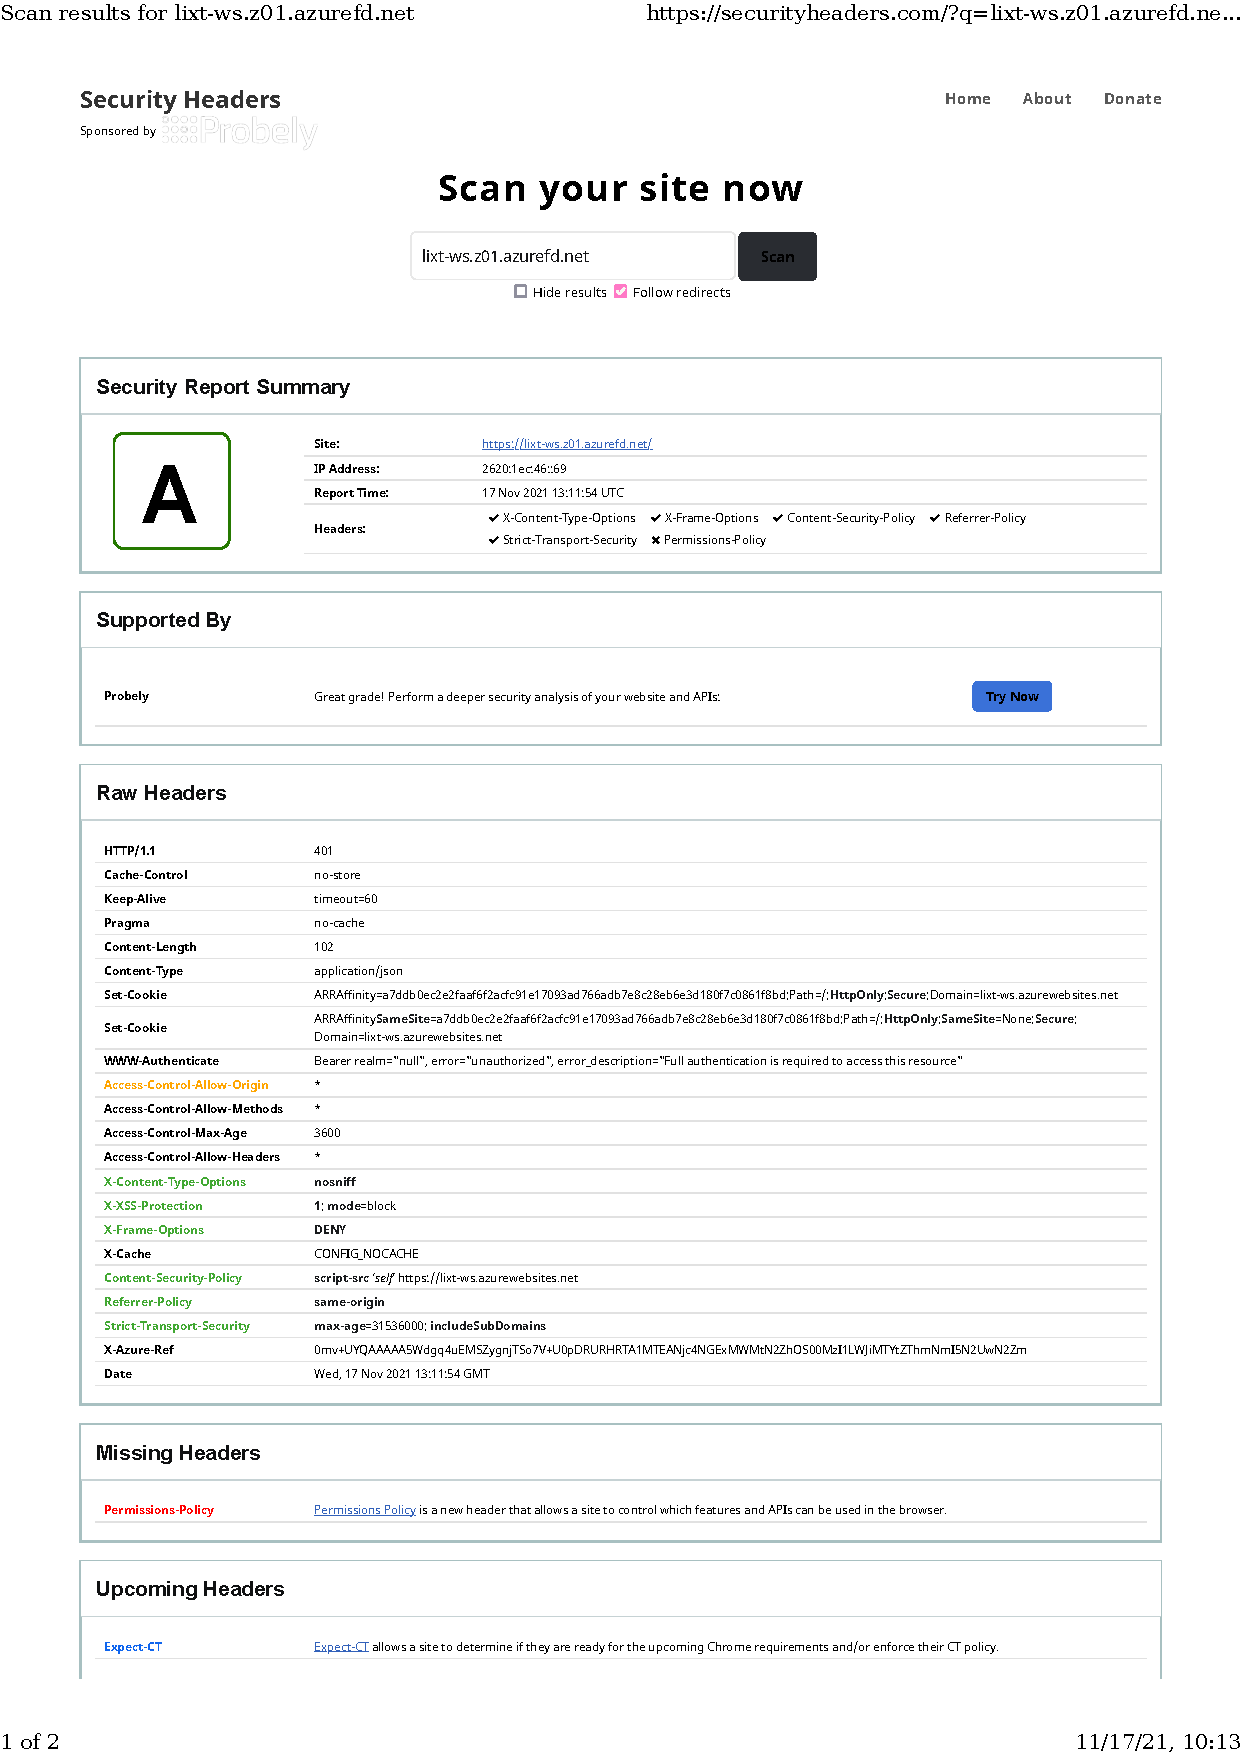
\includepdf[
  pages=1,
  scale=0.7,
  frame=true,pagecommand=\chapter{Métricas do Servidor}
  \label{apx:security_headers_nota}
]{apendices/metricas-seguranca.pdf}
\includepdf[
  pages=2,
  scale=0.8,
  frame=true,
  pagecommand={}
]{apendices/metricas-seguranca.pdf}

\end{apendicesenv}
% ---
